% !TeX program = xelatex
\documentclass[11pt, a4paper, UTF8, fontset=fandol]{ctexart}

\usepackage{amsmath, amssymb}
\usepackage{booktabs, multirow, array, longtable}
\usepackage{threeparttable}
\usepackage{graphicx}
\usepackage{geometry}
\usepackage{tikz}
\usetikzlibrary{positioning, arrows.meta, shapes.geometric, calc, fit, backgrounds, decorations.pathmorphing, shadows}
\usepackage{hyperref}
\usepackage{float}
\usepackage{algorithm}
\usepackage{algorithmic}
\renewcommand{\algorithmicrequire}{\textbf{输入:}}
\renewcommand{\algorithmicensure}{\textbf{输出:}}
\geometry{left=2.3cm, right=2.3cm, top=2.5cm, bottom=2.5cm}
\hypersetup{colorlinks=true, linkcolor=black, citecolor=black, urlcolor=blue}

% 兼容部分 pdflatex 环境中 CJK 粗体字体缺失问题
\makeatletter
\renewcommand{\bfdefault}{m}
\makeatother

\ctexset{ section={format=\Large\rmfamily}, subsection={format=\large\rmfamily}, subsubsection={format=\normalsize\rmfamily} }

\begin{document}
% 手工标题区：避免 \maketitle 默认粗体中文触发字体缺失
\begin{center}
    {\Large TEE 锚定准入与信任流驱动的边缘可信联邦学习\par}
    \vspace{4pt}
    {\large Trust-Flow-Driven Trusted Federated Learning with TEE-Anchored Admission in Edge Computing\par}
    \vspace{10pt}
    {周家凯，步超\par}
    \vspace{2pt}
    {天津理工大学计算机科学与工程学院，中国天津\par}
\end{center}

\begin{abstract}
    联邦学习必须同时回答两个问题：更新是否来自可接受的执行流程，以及更新在 Non-IID 数据下是否有用且语义安全。静态 TEE 准入无法回答第二个问题，单一更新质量阈值又可能误除合法长尾客户端。本文提出 Trust Flow 系统级决策框架，在聚合前分离执行可信度、当轮更新内容、长期效用和短期风险。TEE 锚定的可信管理与证明代理（TMAA）提供准入证据；显式 Kalman 递推和双流 Beta/EMA 状态模型处理冷启动与跨轮行为；按层规则执行风险相关裁剪和按数据量的幸存权重重归一化。实验使用两个 Intel/AMD TEE 能力硬件配置、Flower/PyTorch、CIFAR-10、20 个准入客户端、每个平台 5 个种子和 6 类并发攻击。目标 ASR 对触发器、干净标签和语义攻击取宏平均，无目标攻击则通过干净准确率、损失和状态转移评估。在给定协议下，Trust Flow 达到 92.31\% 干净准确率和 10.21\% 目标 ASR，测试运行中没有永久误封。
\end{abstract}

关键词：联邦学习；边缘计算；可信执行环境；风险状态建模；分层鲁棒聚合；后门防御

\section{引言}
当前，随着终端设备所具备的计算能力愈加强大，越来越多的终端设备能够高效地利用本地数据支持本地模型训练，同时，为更好地以聚合多终端训练经验以支持多方模型协同优化并保护各设备的本地数据隐私，联邦学习范式被深入研究\cite{kairouz2021flsurvey}，其所具备的数据不出本地仅通过模型参数交换的特性被广泛应用于模型的分布式协同训练场景，已然成为边缘智能发展的关键支撑技术。然而，随着万物互联构成的网络环境愈加开放，基于联邦学习的经验聚合以促进模型协同优化所面临的性能瓶颈不再局限于模型结构和优化器设计层面，聚合阶段的可信性和稳健性日益成为影响整体可用性的关键因素。因为在实际应用场景中，不仅各边缘设备端的数据分布具有异构性且处理能力也有显著差异，另外，模型协同优化的各参与方相关行为也难以完全约束，这些特征在经验聚合时显然会放大统计偏移和带来安全风险。

在通常的联邦学习范式中，客户端完成本地数据处理及本地模型训练后，会将模型相关参数上传，服务端聚合各客户端模型参数后会下发更新后的模型参数，以此通过多轮迭代直至收敛，显然，上述流程在实际愈加开放的万物互联多边缘网络环境下，面临着多重风险。具体来说，首先，开放的训练环境缺少强制完整性约束，恶意客户端可以绕过真实训练而直接构造并上传模型参数，也会极大地影响服务端对聚合参数真实性的判断能力，一些研究工作提出了基于可信执行或可验证训练的方法\cite{lu2025tmt,zhang2025rppfl,r1_tee_integrity}，以硬件远程证明等方式保证客户端对模型训练的真实性，但仍然缺乏应对训练过程真实而模型更新却嵌入恶意特征等手段。其次，恶意客户端实施参数投毒、隐蔽后门等攻击\cite{bagdasaryan2020backdoor,wang2019neuralcleanse}，通过将恶意触发特征嵌入常规更新分布参数中，会显著降低单轮检测成功率，一些研究工作提出了基于时序信誉与相似性的方法\cite{cao2021fltrust,fung2020foolsgold}，通过引入跨轮信息来缓解单轮判断的不稳定问题，但对于恶意客户端前期积累信誉后期持续小幅度投毒等潜伏式攻击显然存在识别滞后问题，而且，单一信誉分与固定阈值机制对深层异常触发特征的识别能力也有很大不足。

另外，不同设备的非独立同分布数据（Non-IID）会增加最优更新的方向离散度，很容易模糊正常波动和异常偏移之间的边界，导致强 Non-IID 条件下鲁棒性和泛化性之间的冲突，一些研究工作提出了基于距离排斥或统计截断等的方法抑制异常更新\cite{blanchard2017krum,yin2018byzantine}，还有一些研究工作通过自适应权重调整来缓解异构影响\cite{wang2025rasa}，但强长尾分布情形下，这些方法会将合法偏移的参数更新误判为异常参数，可能导致关键异构信息被过度剔除而显著降低模型泛化能力。在实际场景中，上述执行环境更加开放、跨轮潜伏攻击、强异构统计偏移等挑战往往不会单独出现，尤其是在万物互联的边缘智能场景中，数个因素很可能相互叠加，很容易导致诸如拦截阈值收紧误杀率上升、拦截阈值放宽漏检率增加等多种难以权衡的难题。由此，如何构建覆盖全流程的统一状态建模与联动决策机制，在兼顾客户端本地模型训练的准入及可信和聚合时对客户端低误杀率且高召回率的要求下，维持模型协同优化的收敛和泛化性能成为亟需解决的关键问题。

为应对以上所述的三个主要难题，本文从软硬件协同角度提出一种基于全流程信任流的可信联邦聚合机制。该机制按照联邦学习的执行链路展开：在客户端接入和本地训练阶段，引入 TEE 远程证明、运行特征熵分析与卡尔曼滤波，形成可随轮次更新的动态准入信任分；在服务器审查阶段，基于纯净参考方向计算当轮内容质量，并进一步将客户端状态拆分为历史效用流和瞬时风险流，以贝叶斯后验和风险 EMA 分别刻画长期贡献与短时异常；在聚合阶段，依据上述信任状态执行分层风险门控、幸存者重归一化和动态裁剪，从而在抑制恶意更新的同时保留合法异构贡献，缓解 Non-IID 条件下安全性与泛化性之间的冲突。

本文的主要贡献是明确既有机制的时序与接口，而不是提出新的密码学原语或 Byzantine 估计器：
\begin{enumerate}
    \item \textbf{TEE 锚定准入与冷启动策略}：远程证明限定执行边界，熵观测和带协方差的 Kalman 递推生成动态准入分；新客户端从 NORMAL 开始，首轮证据不能触发不可逆黑名单。
    \item \textbf{双流状态演化}：使用显式衰减 Beta 更新描述历史效用，以最强当轮风险探针的 EMA 保留短期攻击证据，两个流只在计算聚合权限时汇合。
    \item \textbf{风险门控分层聚合}：逐层敏感度决定阈值和裁剪半径，保留原始数据量权重，并仅对幸存权重重归一化。
    \item \textbf{协议匹配的实验评估}：在两个 Intel/AMD TEE 能力平台、5 个平台种子、共享的 5,000 样本客户端训练池与服务器持有的 500 样本 proxy 集、适配后的 CIFAR-10 ResNet-18 和 6 类并发攻击上评估；近期防御仅作研究定位，不赋予未经验证的数值结果。
\end{enumerate}


\section{背景与相关工作}

\subsection{联邦学习与边缘计算协同架构}
联邦学习（Federated Learning, FL）在“数据不出本地”的约束下，通过参数协同完成全局模型训练。在边缘计算场景中，端-边-云（Client-Edge-Cloud）的架构模式已被广泛采用：边缘侧负责本地训练并上传更新，中心服务器负责聚合与模型下发。

在标准的 FL 设置中，全局优化目标为最小化所有客户端数据分布上的经验风险：
\begin{equation}
    \min_{W} \mathcal{L}(W) = \sum_{k=1}^K p_k \mathcal{L}_k(W)
\end{equation}
其中 $p_k = |\mathcal{D}_k| / \sum |\mathcal{D}_j|$ 为数据量占比。在第 $t$ 轮，服务器下发全局模型 $W_{global}^{(t-1)}$，客户端 $k$ 以其为初值在本地数据上执行 $E$ 轮学习率为 $\eta_l$ 的 SGD，得到本地更新：
\begin{equation}
    \Delta W_{k}^{(t)} = W_{k, E}^{(t)} - W_{global}^{(t-1)}, \quad \text{其中 } W_{k, e}^{(t)} = W_{k, e-1}^{(t)} - \eta_l \nabla \mathbb{E}[\ell(W_{k, e-1}^{(t)}; x, y)]
\end{equation}
其中，期望 $\mathbb{E}[\cdot]$ 表示对本地数据集 $\mathcal{D}_k$ 的 mini-batch 采样期望。随后，客户端上传更新量，服务器执行某种形式的参数聚合：$W_{global}^{(t)} = W_{global}^{(t-1)} + \mathrm{Agg}(\{ \Delta W_{k}^{(t)} \}_{k\in\Phi})$。

但是该架构天然存在通信延迟、设备异构和数据 Non-IID 等问题。为缓解这些挑战，已有研究提出簇式联邦（Clustered FL）\cite{r9_clustered}、自适应剪枝扩展（FedPE）\cite{fedpe} 和拆分式联邦（ParallelSFL）\cite{parallelsfl} 等方法。但随着系统复杂度提升，攻击面也随之扩大，恶意节点也更易潜伏并影响训练过程。

\subsection{边缘伪装、模型投毒与隐蔽后门攻击}
在开放且缺少强制准入的联邦网络中，服务器难以准确判断客户端身份与更新质量，攻击手段主要分为两类：其一是\textbf{无目标投毒}（Untargeted Poisoning），如 Sign-flipping 与 Gradient Scaling，目标是破坏全局收敛并造成拒绝服务；其二是\textbf{目标后门攻击}（Targeted Backdoor），如标签翻转、干净标签污染和语义后门，通过隐蔽触发器在推理阶段诱导定向误分类。

\subsection{现有主动防御防线的机制与不可调和的局限性}
为应对上述威胁，早期防御多依赖几何统计过滤，例如 Krum\cite{blanchard2017krum} 与 Trimmed Mean\cite{yin2018byzantine}。近期的研究进一步引入了时序信任评估，如 FLTrust\cite{cao2021fltrust}、FoolsGold\cite{fung2020foolsgold} 与 RaSA\cite{wang2025rasa}，并在恶意检测\cite{dou2025toward}、可信训练框架\cite{lu2025tmt}、分级保护\cite{wang2024federated} 等方向持续扩展。针对后门与合谋攻击，也已有 FLPurifier\cite{flpurifier}、RoseAgg\cite{roseagg} 和 ShieldFL\cite{shieldfl} 等方案。
但纯软件防御在强 Non-IID 与高权限攻击下仍有明显短板：阈值收紧会抬高误杀率（FPR），阈值放宽又可能放过潜伏攻击；同时，当攻击者控制底层环境时，缺少硬件信任根的软件探针难以形成完整闭环。

\subsection{联邦环境下的可信硬件信任根 (TEE)}
为补齐物理可信的缺口，研究开始引入 Intel SGX、ARM TrustZone 等可信执行环境（TEE）。TEE 通过隔离执行与受保护内存保证关键代码和密钥材料的完整性，即便宿主操作系统被攻陷，攻击者也难以直接篡改证明流程\cite{zhang2025rppfl,liao2024verifiable}。现有的工作表明，TEE 在训练完整性\cite{r1_tee_integrity}、威胁缓解\cite{r5_tee_mitigating} 和工业 IoT 信任共享\cite{r12_iot_tee} 中具备现实价值，其在 SGX 环境下的联邦扩展与效率优化也得到验证\cite{xu2021distributed,yan2024efficient}。
本文在此基础上构建软硬件协同防御体系。与仅做静态加密或单维异常评测的方法不同，本文将硬件远程证明（Remote Attestation）与双流信誉演化进行时序耦合：云端负责参数审查，边缘侧 TMAA 提供可信证据与运行时监测，实现“强制准入 + 动态熔断”的联动防护。


\section{系统模型与问题定义}

\subsection{端边云协同架构与系统流转建模}
本文考虑一个典型的端-边-云（Client-Edge-Cloud）异构通信环境（见图~\ref{fig:system_arch}）。系统由中心\textbf{聚合服务器（Server, $\mathcal{S}$）}与 $K$ 个边缘客户端组成，记为 $\mathcal{C}=\{c_1, c_2, \dots, c_K\}$。客户端可能动态上下线，且部分节点可能被攻击者控制。

\begin{figure}[htbp!]
    \centering
    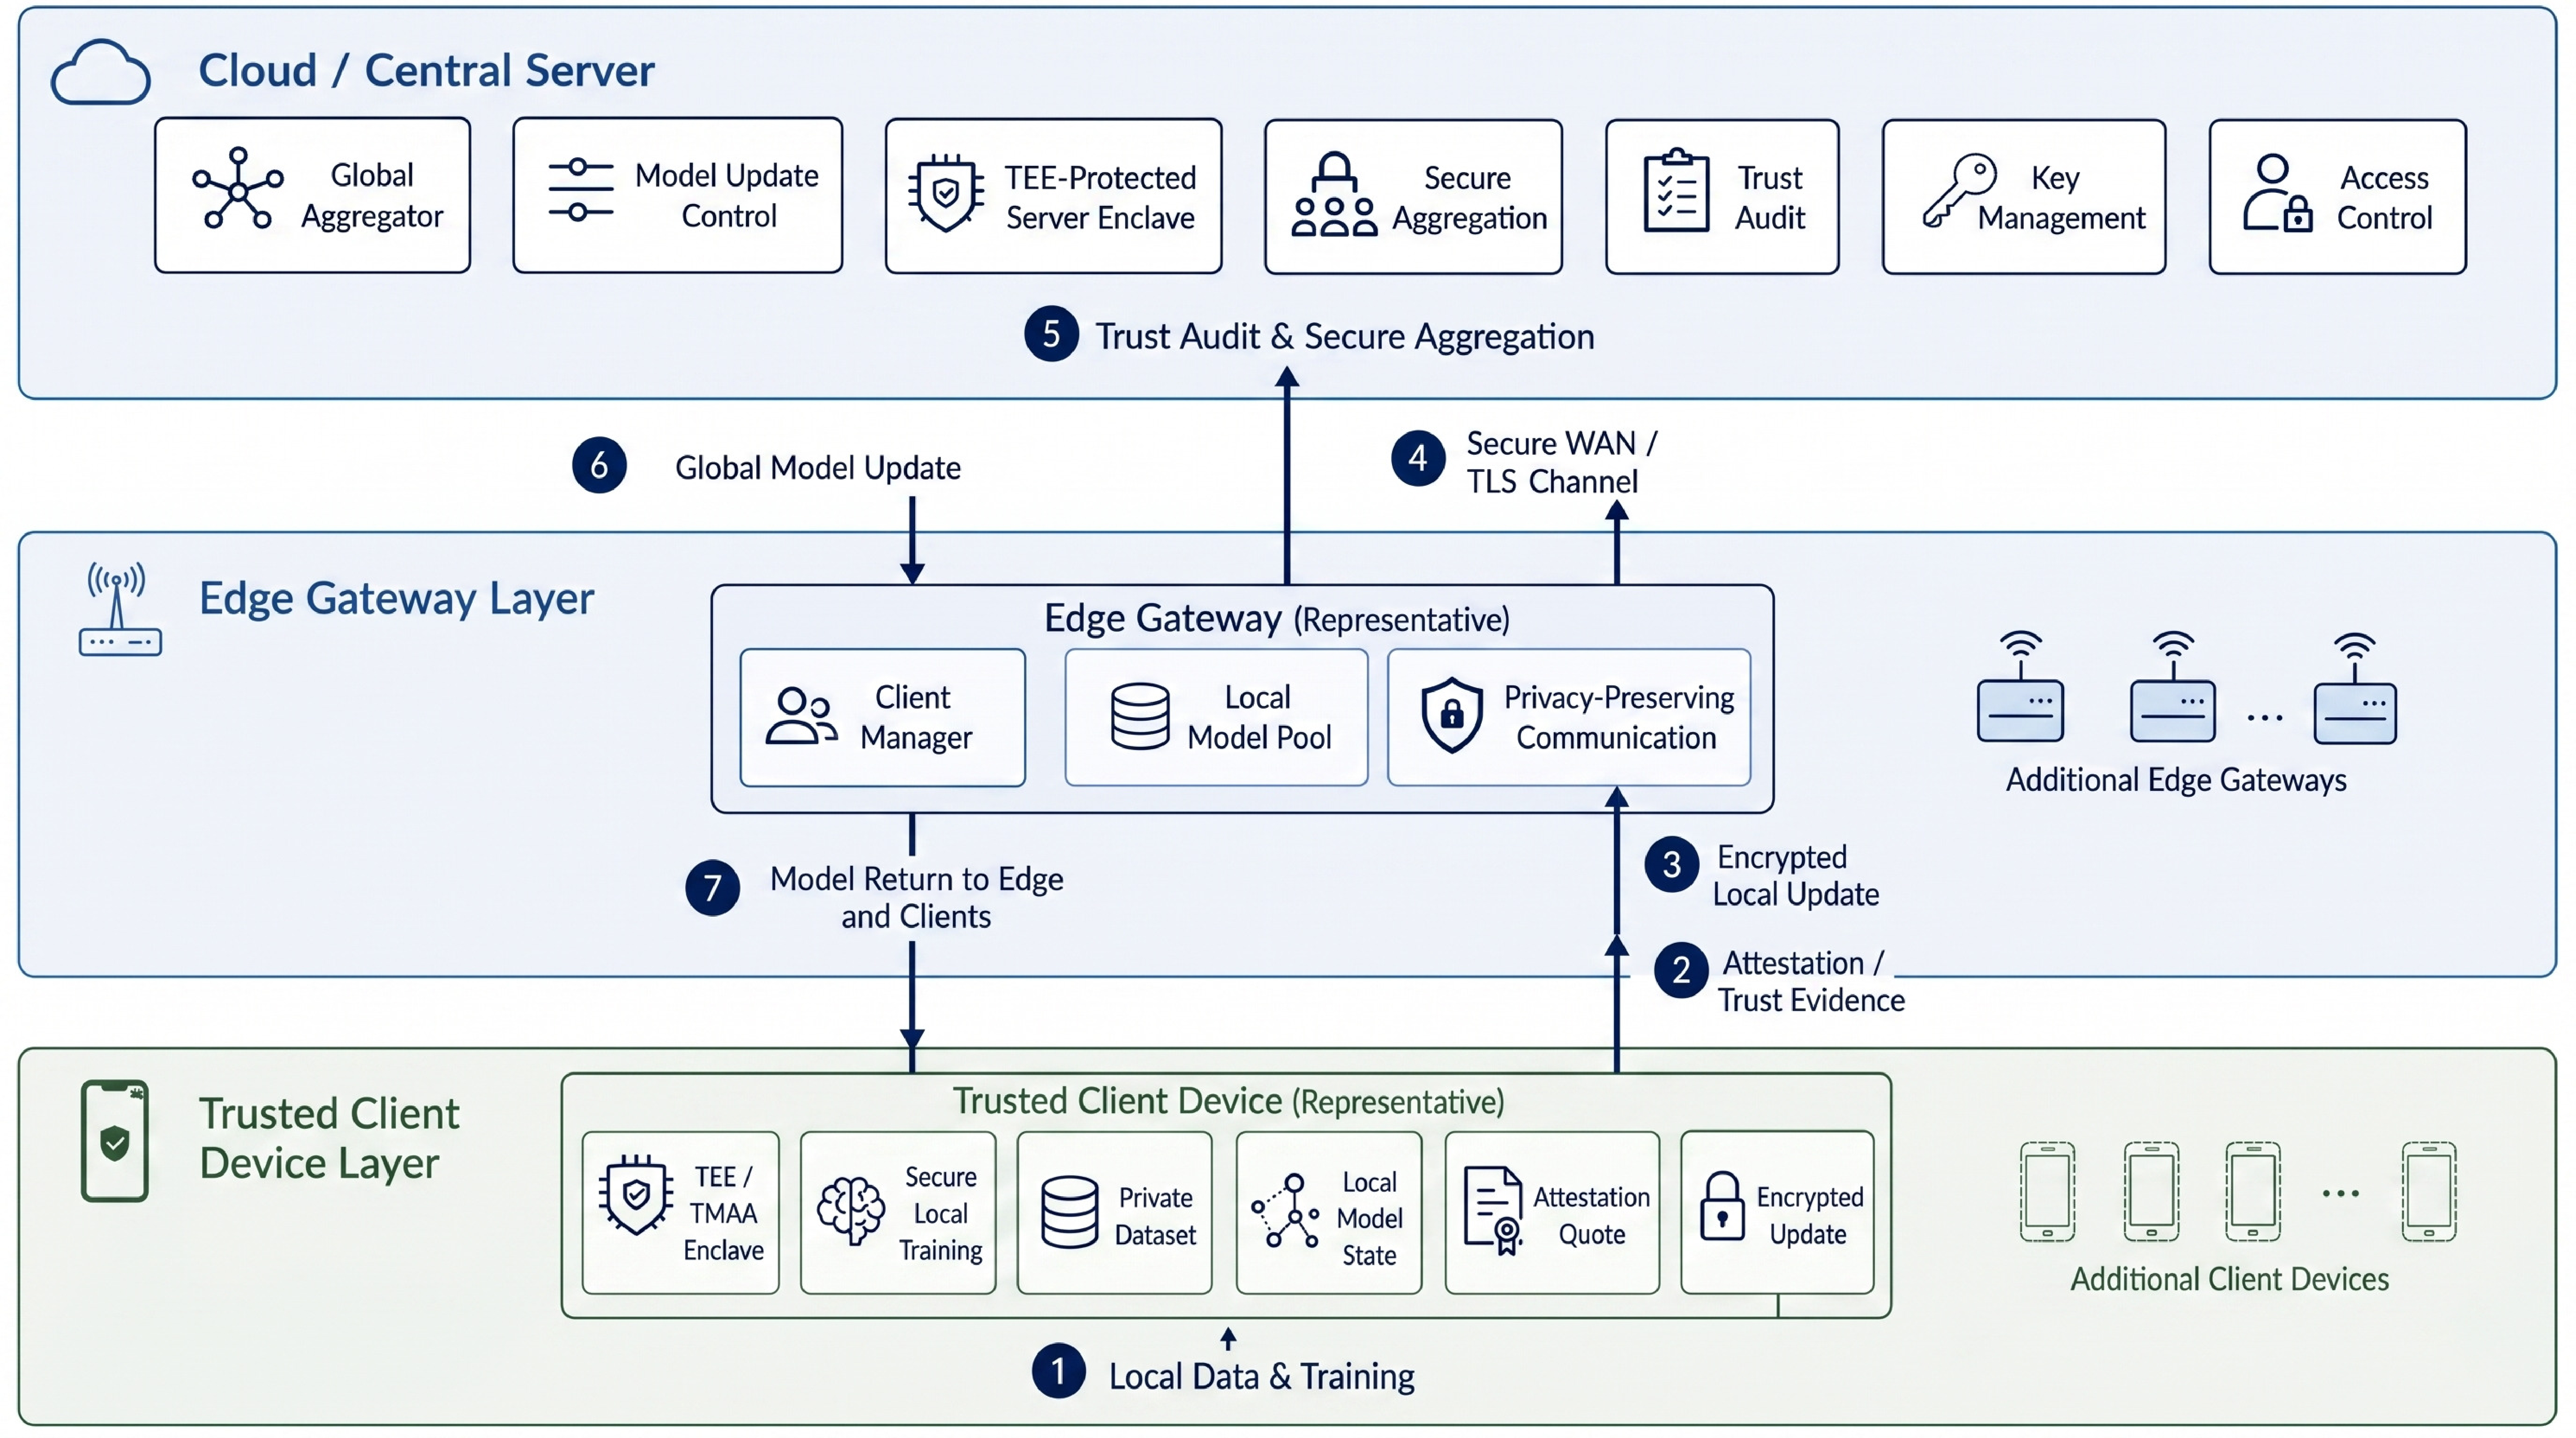
\includegraphics[width=0.90\textwidth]{fig1_system_arch.pdf}
    \caption{联邦计算网络交互：TEE 锚定的端边云协同架构}
    \label{fig:system_arch}
\end{figure}

基于上述网络交互拓扑，本文提出的信任流驱动可信联邦框架在端云之间构建了一条完整的信任传递与评估链路。系统的整体工作流程与主要物理实体模块的相互关系定义如下：

\begin{enumerate}
    \item \textbf{边缘客户端侧（可信执行与特征提取）}：每个接入的客户端需配备可信执行环境（TEE）及部署其内的可信管理代理（TMAA）。在本地训练阶段，TMAA 不仅负责在训练前生成远程证明报告（Attestation Quote）以静态验证执行环境的完整性，还会持续监测训练过程中的关键行为特征序列（如梯度方向变化、损失值波动等）。随后，利用信息熵和卡尔曼滤波进行初步的动态信任评估，连同模型更新参数一并上传至云端。

    \item \textbf{中心服务器侧（审查、演化与聚合控制）}：服务器作为全局协调者，接收到客户端的更新及信任证明后，执行基于信任流的三阶联动防御。首先进行\textbf{内容审查}，提取纯净参考方向并利用余弦相似度计算高维更新质量；其次进入\textbf{双流状态演化}，利用 Beta 贝叶斯推断建立历史效用流以评估长期贡献，并结合多维最大值探针更新瞬时风险流以识别突发异常；最后执行\textbf{分层鲁棒聚合}，根据不同网络层的安全敏感度进行差异化门控裁剪与幸存者权重重归一化，得到筛选后的全局更新并下发。
\end{enumerate}

通过上述端与云实体模块的协同交互，系统实现了“硬件门禁准入 $\to$ 运行特征监测 $\to$ 信任状态演化 $\to$ 风险门控聚合”的全生命周期物理与逻辑流转闭环。


\subsection{复合型威胁假设与信任边界 (Threat Model)}
为清晰界定攻防能力边界，本文采用如下威胁模型（见图~\ref{fig:threat_model}）：
\begin{itemize}
    \item \textbf{TEE 信任边界}：Intel 和 AMD TEE 能力平台保护证明关键代码、设备密钥、报告完整性、报告新鲜度和可信监测路径，使其免受受攻陷宿主操作系统的篡改；但 TEE 不认证标签、样本、优化目标或语义意图。因此，攻击者可以在有效测量的训练流程内部生成带签名的投毒更新，而证明完成后在受保护路径之外篡改更新则被排除。
    \item \textbf{诚实但好奇服务器}：服务器遵循双流评分与分层聚合协议，可以看到单个更新和审计统计量，但不能改变规定的状态转移规则。
    \item \textbf{内部恶意客户端}：恶意客户端可以执行标签翻转、触发器后门、干净标签投毒、语义投毒、符号翻转和梯度缩放。分析假设恶意准入客户端少于 $50\%$；$50\%$ 实验仅是超出假设范围的压力测试，不构成理论 Byzantine 阈值。物理探测和高级微架构侧信道不在威胁模型中。
\end{itemize}

\begin{figure}[htbp!]
    \centering
    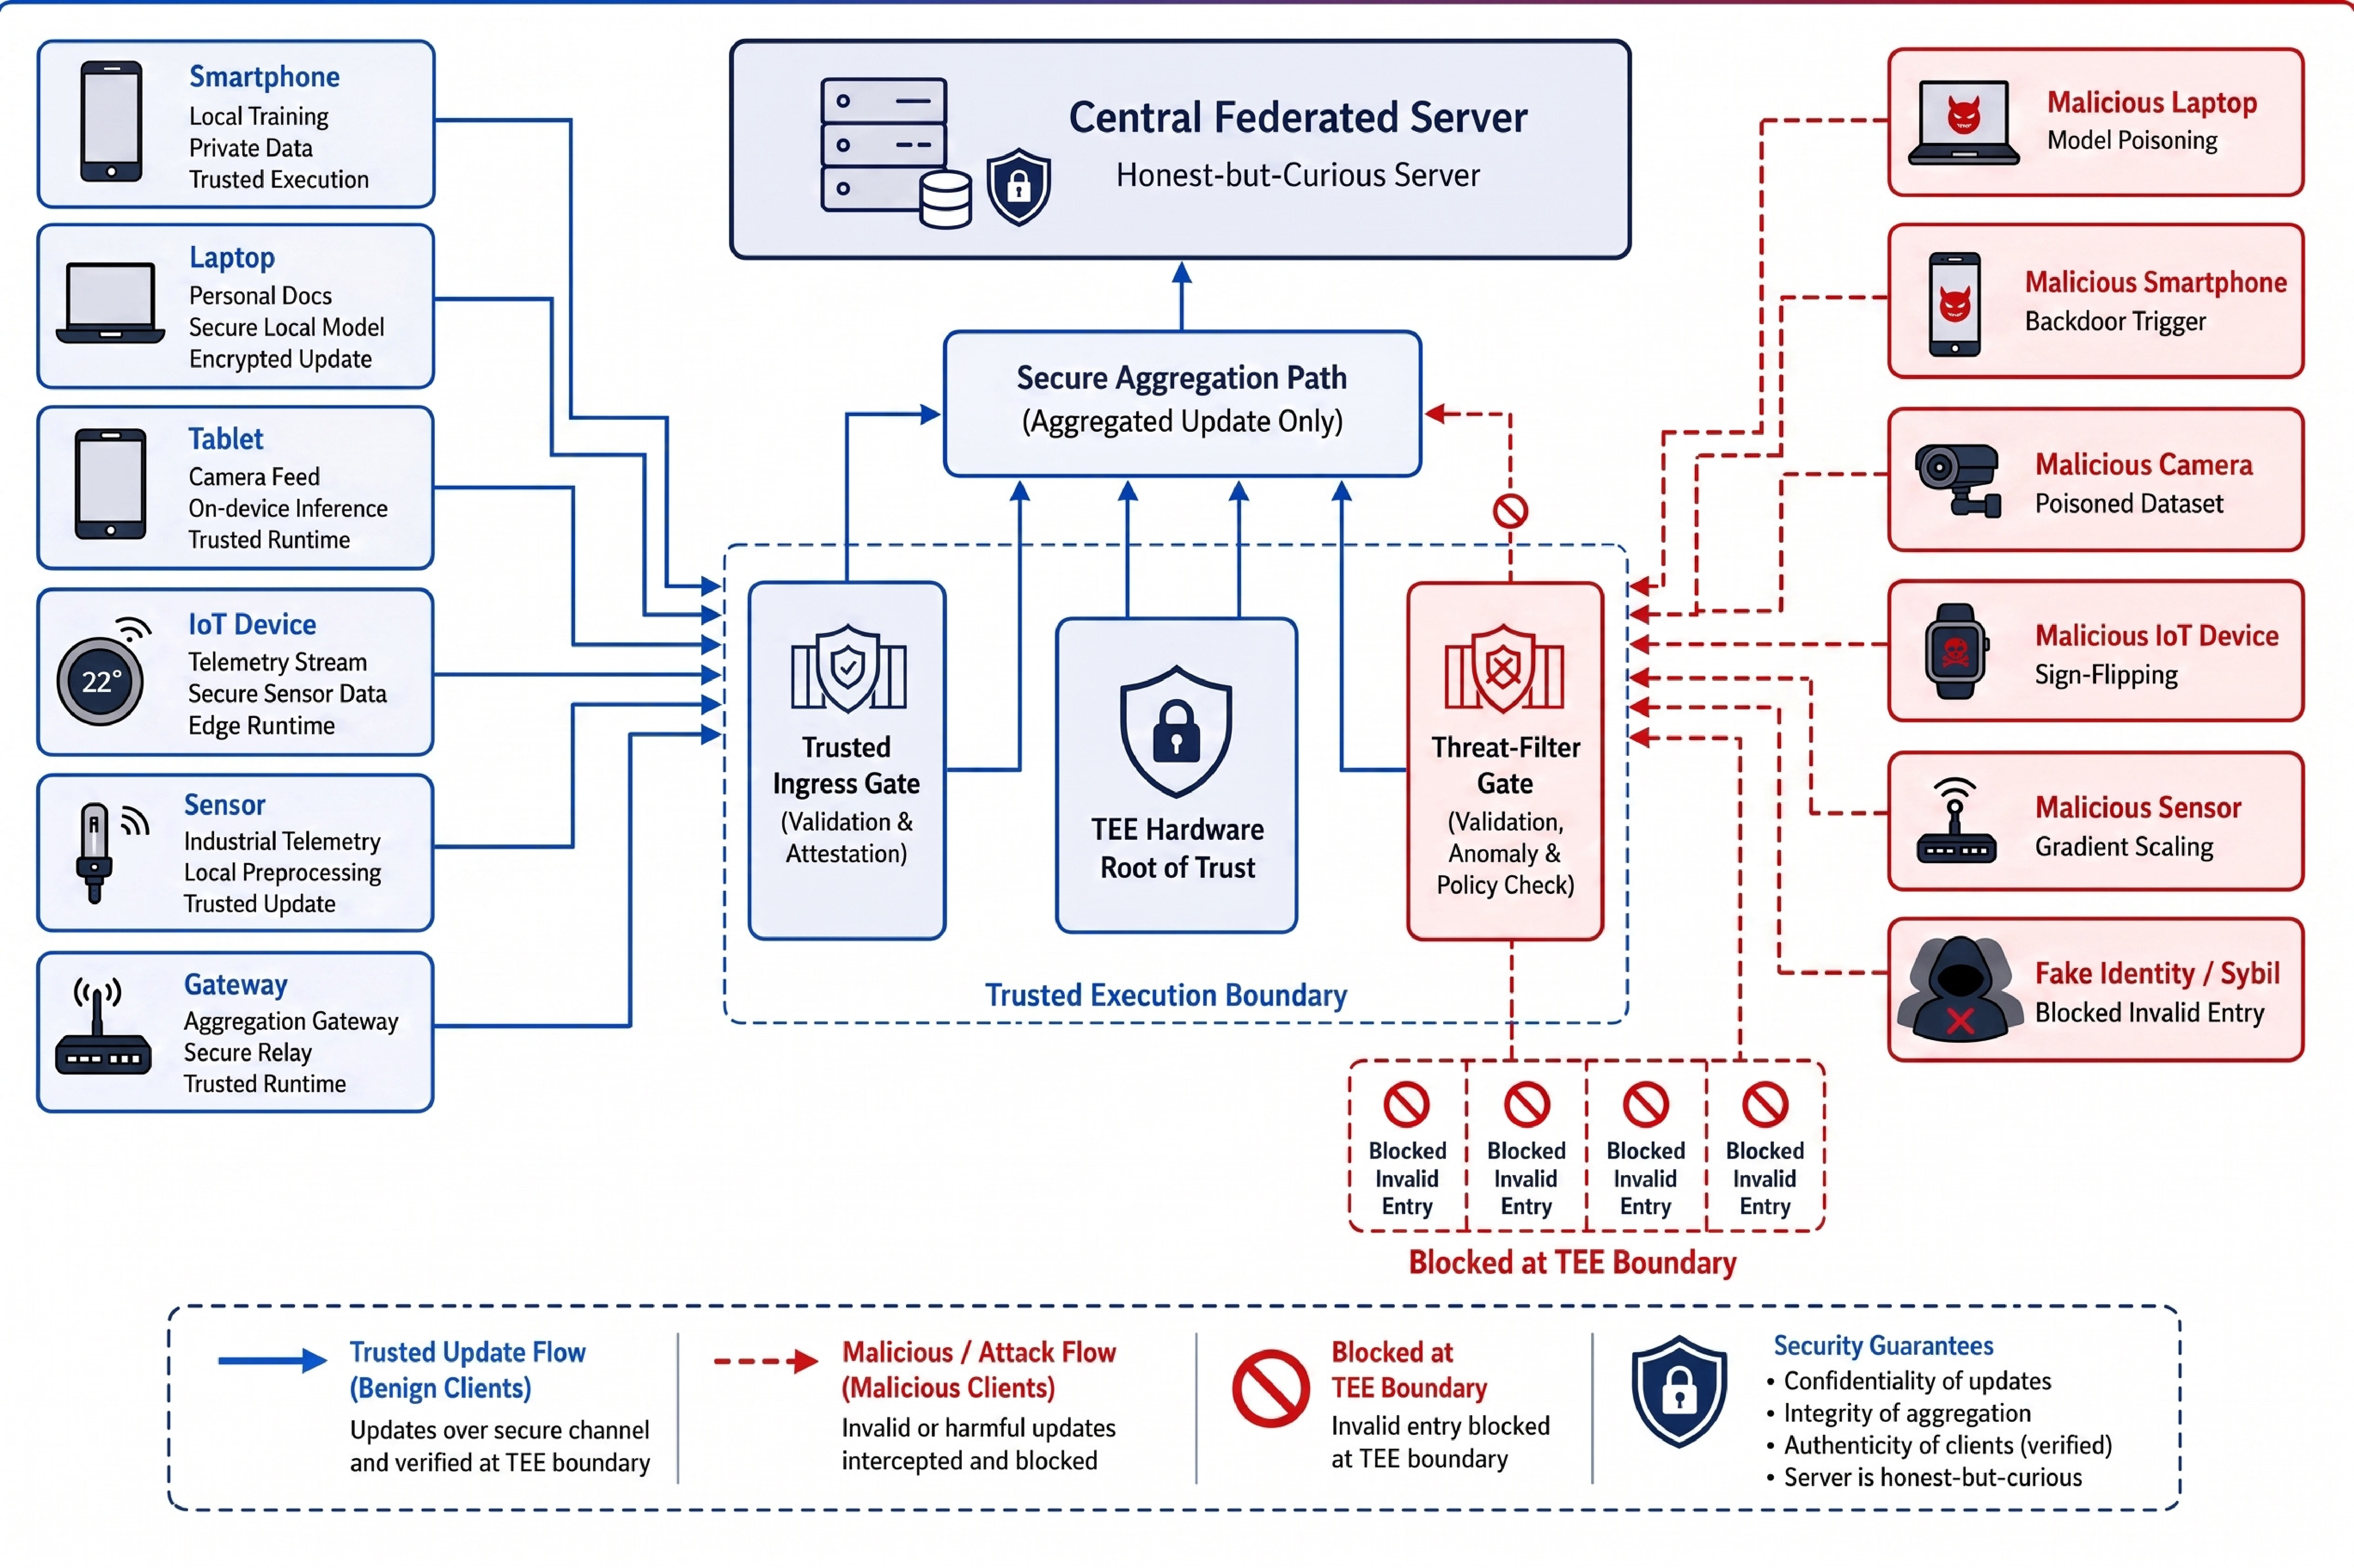
\includegraphics[width=0.88\textwidth]{fig2_threat_model.pdf}
    \caption{边缘广域网络下的安全渗透与多维复合型投毒威胁模型示意图}
    \label{fig:threat_model}
\end{figure}

\subsection{设计目标与系统边界 (Design Goals)}
Trust Flow 旨在在给定攻击下保持收敛，减少长尾客户端的不可逆误封，并按系统边界报告开销：附加 TrustReport 约为 15 KB，服务器聚合与审查时间由 2.10 s 增至 4.85 s，辅助安全路径实测为每个准入客户端每轮约 11 ms，覆盖 enclave 切换、内存压力和密码学聚合路径的开销；设备侧 TEE Quote 生成、签名和轻量监测另行实测为每个准入客户端每轮约 12--15 ms。完整端到端通信延迟和厂商特定证明延迟不在本文报告的测量范围内。本文不将该流程称为 secure aggregation，因为服务器必须检查单个客户端的证据；辅助安全路径与主协议分开报告。


\section{本文方法：信任流驱动的可信联邦框架}

针对上述威胁模型，本文提出“信任流驱动的可信联邦学习”框架（见图~\ref{fig:framework}）。从联邦学习的执行次序看，该框架先在客户端侧完成可信准入和运行监测，再在服务器侧完成当轮内容审查与跨轮信誉演化，最后进入聚合阶段的分层安全控制。由此，每一轮训练被划分为四个决策阶段：准入与运行监测、内容审查、状态演化和分层聚合；全局模型下发作为协议输出随后执行。若进一步抽象，可对应为“客户端准入与监测、服务器审查与演化、聚合安全保障”三个层次。

这种“总-分”结构的核心在于信任状态的连续传递。阶段一输出 $TrustScore$，回答客户端是否具备可信接入和可信执行基础；阶段二输出 $ContentScore$，判断本轮上传更新是否偏离纯净参考和群体协作方向；阶段三将当轮信号沉淀为 $HistPerf$ 与 $RiskEMA$，区分长期低贡献和短时高风险；阶段四再把三类信号融合为 $RawScore$，并按网络层执行差异化聚合。不同于单点防御，每阶段产生的数据会在后续阶段继续发挥约束作用，持续更新\textbf{信任流（Trust Flow）}并形成闭环控制。

\begin{figure}[htbp]
    \centering
    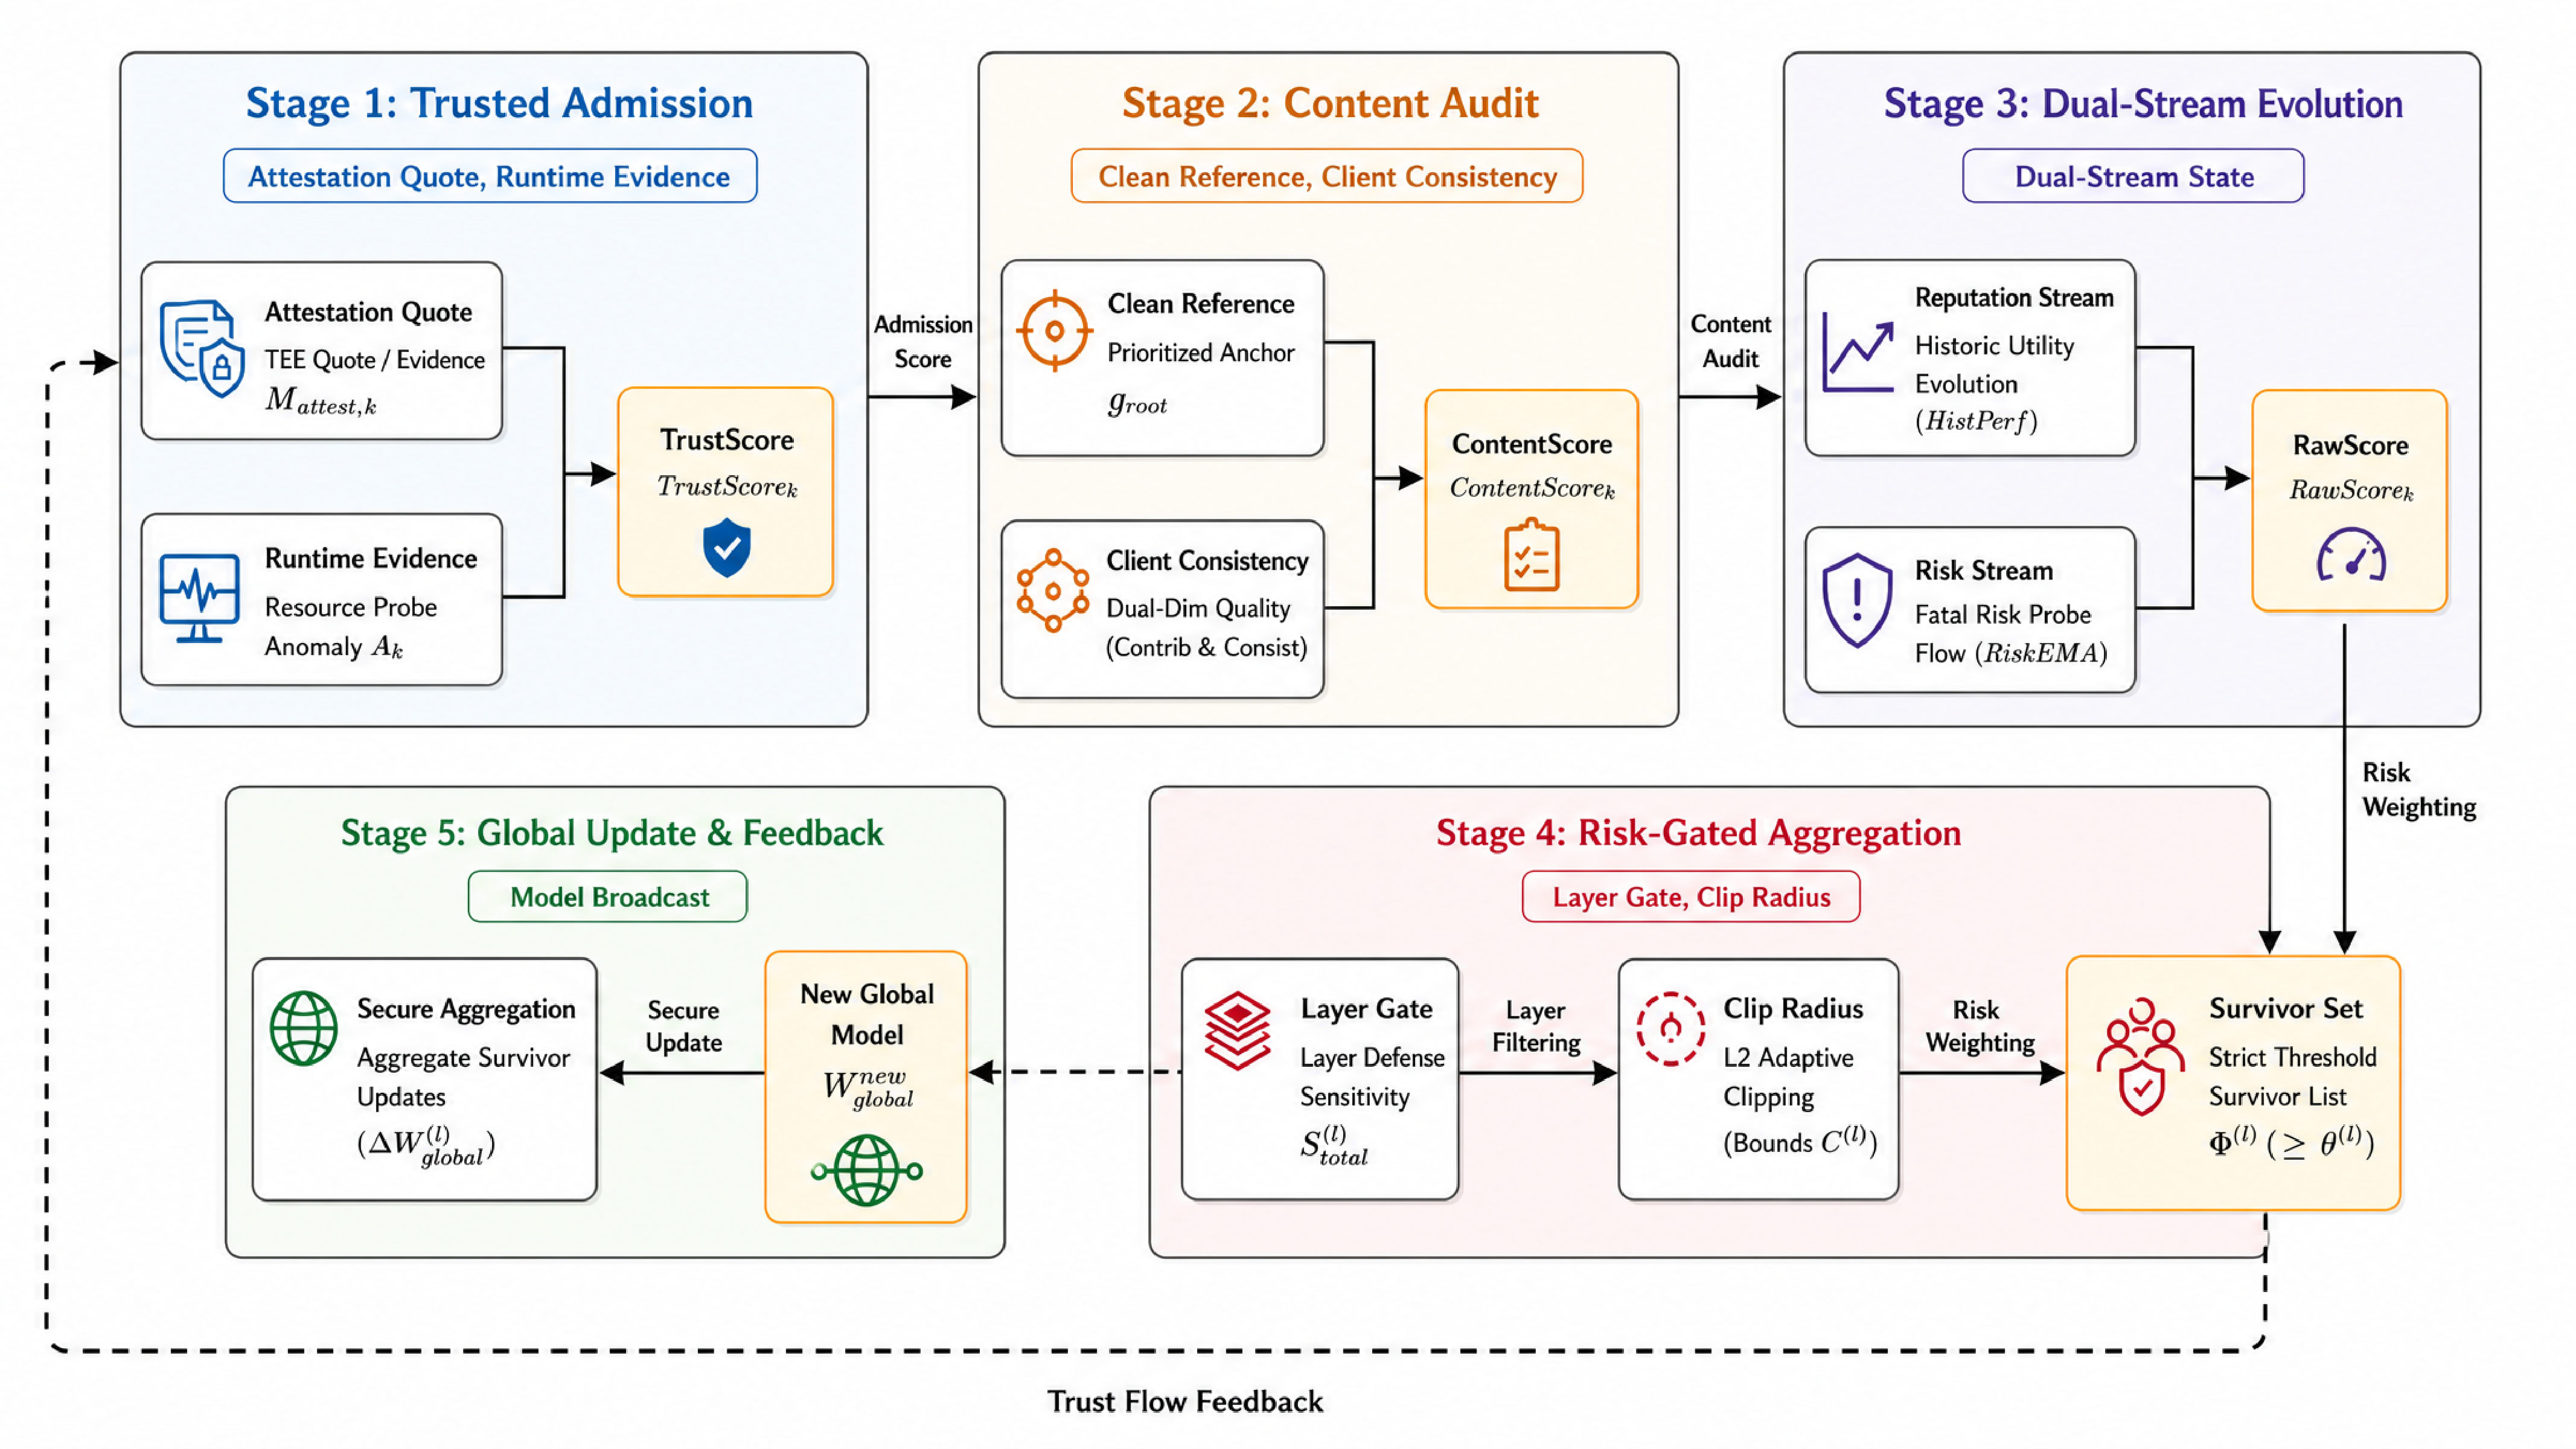
\includegraphics[width=\textwidth]{fig3_arch.pdf}
    \caption{信任流驱动的可信联邦学习四阶段防御闭环架构总览}
    \label{fig:framework}
\end{figure}

为便于后续推导，表~\ref{tab:notations} 给出核心符号定义。

\begin{table}[htbp]
    \centering
    \caption{核心系统参数与信任流符号定义}
    \label{tab:notations}
    \renewcommand{\arraystretch}{1.25}
    \setlength{\tabcolsep}{3pt}
    \begin{tabular*}{\textwidth}{@{\extracolsep{\fill}} >{\raggedright\arraybackslash}p{2.8cm} >{\raggedright\arraybackslash}p{4.5cm} >{\raggedright\arraybackslash}p{2.2cm} >{\raggedright\arraybackslash}p{4.5cm}}
        \toprule
        \textbf{符号} & \textbf{定义描述} & \textbf{符号} & \textbf{定义描述} \\
        \midrule
        $W_{global}^{(t)}$ & 第 $t$ 轮的全局模型权重 & $\mathcal{A}$ & 本轮具备有效聚合资格的活跃节点集合 \\
        $\Delta W_k$ & 客户端 $k$ 提交的模型梯度/参数更新 & $\Phi^{(l)}$ & 第 $l$ 层的有效安全幸存者子集 \\
        $TrustScore_k$ & TEE 硬件锚定的准入基础信任分 & $HistPerf_k$ & 历史效用流累积状态 ($HistPerf \in [0, 1]$)\\
        $ContentScore_k$ & 双参比下的当轮内容质量得分 & $RiskEMA_k$ & 瞬时风险流衰减状态 ($RiskEMA \in [0, 1]$)\\
        $RawScore_k$ & 融合三维得分并施加风险折扣的最终权限分 & $M_{attest,k}$ & 硬件远程证明 (Attestation) 验证通过标志 \\
        $g_{root}$ & 服务器提取的纯净指导锚点方向 & $A_k$ & 客户端 $k$ 的物理资源运行时异常分数 \\
        \bottomrule
    \end{tabular*}
    \renewcommand{\arraystretch}{1.0}
\end{table}

\subsection{硬件准入与动态信任评估}
准入由静态执行准入和动态证据跟踪两部分组成。令
$M_{\mathrm{attest},k}\in\{0,1\}$ 表示证明报告、随机数新鲜度以及报告与本轮和更新摘要绑定是否有效。初始化时，客户端调用设备唯一密钥并生成 quote，其中包含厂商相关测量摘要、代码身份、运行配置、轮次随机数、更新摘要和单调新鲜度计数器。未通过检查的客户端在其更新进入统计聚合前被拒绝。

本地训练期间，可信管理与证明代理监测标准化序列
$\mathcal{X}_k^{(t)}=\{\Delta\mathrm{grad},\Delta\mathrm{loss},
\mathrm{instr\_dist}\}$。拼接标准化特征直方图后，令
$h_k^{(t)}=H(\mathcal{X}_k^{(t)})/H_{\max}\in[0,1]$。熵导出的观测方差和观测值定义为
\begin{equation}
    R_k^{(t)}=\exp(\lambda h_k^{(t)}),\qquad
    Z_k^{(t)}=\operatorname{clip}\!\left(
    w_aM_{\mathrm{attest},k}+(1-w_a)(1-h_k^{(t)}),0,1\right),
\end{equation}
其中 $w_a=0.7$，$\lambda=1.0$。高熵只表示证据不确定性增加，并不直接等价于恶意标签。

标量 Kalman 递推为
\begin{equation}
    T_k^{-,(t)}=T_k^{(t-1)},\qquad P_k^{-,(t)}=P_k^{(t-1)}+Q,
\end{equation}
\begin{equation}
\begin{aligned}
    K_k^{(t)}&=\frac{P_k^{-,(t)}}{P_k^{-,(t)}+R_k^{(t)}},\\
    T_k^{(t)}&=T_k^{-,(t)}+K_k^{(t)}
        \left(Z_k^{(t)}-T_k^{-,(t)}\right),\\
    P_k^{(t)}&=(1-K_k^{(t)})P_k^{-,(t)}.
\end{aligned}
\end{equation}
其中 $Q=0.01$ 是固定过程噪声方差。新准入客户端初始化为
$T_k^{(0)}=1$、$P_k^{(0)}=0.25$ 和 $RiskEMA_k^{(0)}=0$，准入权限为
\begin{equation}
    TrustScore_k^{(t)}=M_{\mathrm{attest},k}
    \operatorname{clip}\!\left(\frac{T_k^{(t)}}{1+P_k^{(t)}},0,1\right).
\end{equation}
高熵会降低 Kalman 增益，防止不确定观测突然改写跨轮信任。有效证明后的新客户端从 NORMAL 状态开始，首轮证据只能降低当前更新权限，不能触发不可逆黑名单。

\subsection{参考方向构建与一致性审查}
仅依赖客户端之间的余弦相似度容易被合谋攻击误导。本文优先使用服务器明确声明的 clean reference：报告实验中的 500 个均衡 proxy 样本（每类 50 个）由服务器持有，绝不进入客户端训练，并按照同一协议提供给所有依赖参考集的基线，同时用于指导梯度、干净损失和激活探针。若该方向不可用，则由高信任、低风险的准入客户端更新构造回退参考。其权重定义为：
\begin{equation}
    \omega_{k}^{ref} = TrustScore_{k} \cdot (1 - RiskEMA_{k}^{prev})^{2}.
\end{equation}
最终参考方向 $g_{root}$ 为：
\begin{equation}
    g_{root}=
    \begin{cases}
        g_{root\_clean},                                                      & \text{若服务器验证集方向可用}, \\
        \sum_{k} \frac{\omega_{k}^{ref}}{\sum_j \omega_{j}^{ref}} \Delta W_k, & \text{否则}.
    \end{cases}
\end{equation}

在得到 $g_{root}$ 后，服务器对每个客户端更新 $\Delta W_k$ 计算内容质量分。该分数同时考虑全局贡献（与参考方向一致性）和群体一致性（与其他高信誉客户端一致程度）：
\begin{align}
    S_{contrib,k}    & = \max\left(0,\ \alpha_{1} + \alpha_{2} \cdot \cos(\Delta W_{k}, g_{root})\right),                                                                                             \\
    S_{consist,k}    & = \frac{\sum_{j\neq k} TrustScore_{j} \cdot \max\left(0,\ \alpha_{1} + \alpha_{2} \cdot \cos(\Delta W_{k}, \Delta W_{j})\right)}{\sum_{j\neq k} TrustScore_{j} + \varepsilon}, \\
    ContentScore_{k} & = \frac{(1 + \beta_{fusion}^{2}) \cdot S_{consist,k} \cdot S_{contrib,k}}{\beta_{fusion}^{2}\cdot S_{consist,k} + S_{contrib,k} + \varepsilon}.
\end{align}
其中，$\alpha_1+\alpha_2=1.0$ 用于调节余弦映射区间；$\beta_{fusion}>1.0$（默认 $\beta_{fusion}=2.0$）表示适当提高“与纯净方向一致”的权重，以增强对合谋偏移的抑制能力。$ContentScore_k$ 只描述本轮更新的内容质量，并不直接等同于永久信誉。对于强 Non-IID 场景中的长尾合法节点，单轮低分可能来自数据偏斜而非攻击行为，因此该分数会继续进入阶段三的跨轮状态演化，由历史效用流和瞬时风险流共同决定后续处置。

\begin{algorithm}[htbp]
    \caption{基于 TEE 硬件锚点与纯净参考的准入与内容审查}
    \label{alg:phase12}
    \begin{algorithmic}[1]
        \REQUIRE 客户端集合 $\mathcal{C}$，本轮收到的参数更新 $\{\Delta W_k\}_{k\in\mathcal{C}}$，上轮状态 $RiskEMA^{(t-1)}$
        \ENSURE $TrustScore_k$, $ContentScore_k$, 有效参考基准 $g_{root}$
        \STATE \textbf{第一阶段：硬件锚定与动态信任度量}
        \FOR{每个客户端 $k \in \mathcal{C}$}
        \IF{$M_{attest,k} == 0$ (TEE 远程证明失败)}
        \STATE 拒绝接入：$TrustScore_k \leftarrow 0$，并跳过本轮
        \ELSE
        \STATE \textit{TEE 内部}: 记录行为序列 $\mathcal{X}_k = \{ \Delta \text{grad}, \Delta \text{loss}, \text{instr\_dist} \}$
        \STATE 计算信息熵 $H_k \leftarrow -\sum p(x_i) \log p(x_i)$
        \STATE 将熵映射为测量噪声 $R_k \leftarrow \exp(\lambda \cdot H_k)$
        \STATE \textit{卡尔曼滤波更新}:
        \STATE 信任估计 $\hat{T}_k$, 协方差 $P_k \leftarrow \mathrm{KalmanFilter}(H_k, \text{前序状态})$
        \STATE 门禁信任分 $TrustScore_k \leftarrow \hat{T}_k \cdot \frac{1}{1 + P_k}$
        \ENDIF
        \ENDFOR
        \STATE \textbf{第二阶段：参考方向构建与协同一致性审查}
        \IF{具备服务器纯净验证集数据}
        \STATE 提取真实指导梯度 $g_{root} \leftarrow g_{root\_clean}$
        \ELSE
        \STATE 计算非线性权重 $\omega_k^{ref} \leftarrow TrustScore_k \cdot (1 - RiskEMA_k^{(t-1)})^2$
        \STATE 生成降级纯净锚点 $g_{root} \leftarrow \sum_k (\omega_k^{ref} \Delta W_k) / \sum_j \omega_j^{ref}$
        \ENDIF
        \FOR{通过准入的活跃客户端 $k$}
        \STATE 全局贡献分 $S_{contrib,k} \leftarrow \max(0, \alpha_1 + \alpha_2 \cos(\Delta W_k, g_{root}))$
        \STATE 群体协作分 $S_{consist,k} \leftarrow \frac{\sum_{j \neq k} TrustScore_j \max(0, \alpha_1 + \alpha_2 \cos(\Delta W_k, \Delta W_j))}{\sum_{j \neq k} TrustScore_j + \varepsilon}$
        \STATE 调和内容分 $ContentScore_k \leftarrow \frac{(1+\beta_{fusion}^2)S_{consist,k} S_{contrib,k}}{\beta_{fusion}^2 S_{consist,k} + S_{contrib,k} + \varepsilon}$
        \ENDFOR
        \RETURN $\{TrustScore_k, ContentScore_k, g_{root}\}$
    \end{algorithmic}
\end{algorithm}


\subsection{历史效用与瞬时风险的双流演化}
单一信誉分会混淆数据偏斜造成的低效用与攻击造成的高风险。因此，
Trust Flow 维护慢速历史效用流和快速当轮风险流。令
$q_k^{(t)}=\operatorname{clip}(ContentScore_k^{(t)},0,1)$，历史流使用衰减
Beta 更新：
\begin{equation}
    a_k^{(t)}=\beta_h a_k^{(t-1)}+q_k^{(t)},\quad
    b_k^{(t)}=\beta_h b_k^{(t-1)}+1-q_k^{(t)},\quad
    HistPerf_k^{(t)}=\frac{a_k^{(t)}}{a_k^{(t)}+b_k^{(t)}+\varepsilon}.
\end{equation}
新客户端从 $a_k^{(0)}=b_k^{(0)}=1$ 开始，因此
$HistPerf_k^{(0)}=0.5$。衰减因子 $\beta_h\in(0,1)$ 在测试前固定。历史流会逐步降低权限，并允许合法长尾客户端恢复。

短期风险流定义为
\begin{equation}
    RiskEMA_k^{(t)}=\beta_rRiskEMA_k^{(t-1)}
    +(1-\beta_r)Risk_k^{inst},
\end{equation}
其中 $Risk_k^{inst}$ 是当轮最大探针。令
$u_k^{(t)}=1-HistPerf_k^{(t)}$、$r_k^{(t)}=RiskEMA_k^{(t)}$，阈值
$(\tau_h,\tau_s,\tau_q,\tau_b)=(0.26,0.64,0.80,0.90)$
分别表示效用缺口、软风险、隔离和黑名单。NORMAL 客户端在连续两轮满足
$u_k^{(t)}>\tau_h$ 或 $r_k^{(t)}\geq\tau_s$ 后进入 SUSPECT。SUSPECT
客户端在连续三轮满足相同条件，或某一轮当前探针满足
$Risk_k^{inst}\geq\tau_q$ 后进入 QUARANTINE。QUARANTINE 客户端在连续
四轮满足 $r_k^{(t)}\geq\tau_b$ 后进入 BLACKLIST。SUSPECT 或 QUARANTINE
恢复需要连续两轮满足 $u_k^{(t)}\leq\tau_h$ 且 $r_k^{(t)}<\tau_s$；
BLACKLIST 在一次实验内不可逆。条件不满足时计数器重置，状态更新在分层
聚合前完成。首轮证据只能降低当前更新权限，不能触发永久黑名单。

两个流只在聚合权限计算时汇合：
\begin{align}
    RawScore_k^{(t)} &=(TrustScore_k^{(t)})^\alpha
    (ContentScore_k^{(t)})^\beta(HistPerf_k^{(t)})^\gamma
    (1-RiskEMA_k^{(t)})^p .
\end{align}
因此，当轮风险可以否决高历史信誉的潜伏攻击，而低相似度的良性长尾
客户端仍可通过慢速流恢复。

\subsection{风险门控驱动的分层聚合}
后门可能集中在深层，而浅层特征仍可能包含有价值的异构信息。Trust
Flow 为每个网络层 $l$ 分配敏感度分数。设网络共有 $L$ 层，定义
\begin{align}
    S_{priv}^{(l)}&=\exp(-\tau_p l/L),\qquad
    S_{util}^{(l)}=\frac{\|g_{root}^{(l)}\|_2}
    {\max_m\|g_{root}^{(m)}\|_2+\varepsilon},\\
    S_{sec}^{(l)}&=\frac{1}{2}\left(1-\frac{1}{|\mathcal{T}|}
    \sum_{k\in\mathcal{T}}\cos(\Delta W_k^{(l)},g_{root}^{(l)})\right).
\end{align}
其中
$\mathcal{T}=\{k\in\mathcal{A}:M_{\mathrm{attest},k}=1,\,
RiskEMA_k^{(t-1)}<\tau_s\}$ 为可信参考集。若该集合为空，服务器仅使用
$\mathcal{A}$ 进行归一化并记录没有可信对等参考。因此
$S_{priv}^{(l)}$、$1-S_{util}^{(l)}$ 和 $S_{sec}^{(l)}$ 均位于 $[0,1]$。
定义
\begin{equation}
    S_{total}^{(l)}=w_pS_{priv}^{(l)}+w_u(1-S_{util}^{(l)})
    +w_sS_{sec}^{(l)},\qquad (w_p,w_u,w_s)=(0.3,0.3,0.4).
\end{equation}
层阈值和裁剪半径为
\begin{equation}
    \theta^{(l)}=\mu_{base}+\lambda_sS_{total}^{(l)},\qquad
    C^{(l)}=\frac{C_{base}}{S_{total}^{(l)}+\varepsilon_c},
\end{equation}
其中 $\tau_p=3.0$，$C_{base}$ 是可信客户端更新范数的中位数。可疑漂移
更强的层更难进入且裁剪更紧。

幸存者集合为
$\Phi^{(l)}=\{k\in\mathcal{A}:RawScore_k^{(t)}\geq\theta^{(l)}\}$。为保留
全局目标中的数据量因素，权重定义为
\begin{equation}
    \tilde{w}_k^{(l)}=
    \frac{p_kRawScore_k^{(t)}}{\sum_{j\in\Phi^{(l)}}p_jRawScore_j^{(t)}
    +\varepsilon},\qquad
    \widehat{\Delta W}_k^{(l)}=
    \frac{\Delta W_k^{(l)}}{\max(1,\|\Delta W_k^{(l)}\|_2/C^{(l)})}.
\end{equation}
最终更新为
$\Delta W_{\mathrm{global}}^{(l)}
=\sum_{k\in\Phi^{(l)}}\tilde{w}_k^{(l)}
\widehat{\Delta W}_k^{(l)}$。若没有客户端幸存，则保留
$RawScore$ 最大的客户端，赋予单位归一化权重，并继续使用同一裁剪半径。
重归一化避免移除风险客户端后有效学习率隐式下降。

\subsection{模型更新下发与知识留存}
分层聚合完成后，服务器将经过筛选的增量应用到全局模型：$W_{global}^{new}=W_{global}^{old}+\Delta W_{global}$，并同步下发更新后的模型及保留的客户端状态（含 $HistPerf$）。该过程闭合了给定协议下的控制回路；收敛与攻击抑制属于实验部分评估的经验性质。

\subsection{双流设计的解释范围}
历史流对良性内容变化起低通滤波作用，最大风险探针与风险 EMA 则保留
突发警告。在有界的良性波动和持续攻击证据下，这种分离解释了长尾客户
端能够恢复、潜伏攻击能够被快速降权的原因。上述结论是给定阈值下的
设计性质，不是保证零 FPR 或普遍 Byzantine 鲁棒性的定理；严格保证仍
需要超出本文经验范围的分布和攻击假设。

\section{实验与分析}
\label{sec:experiments}
\subsection{实验设置与可复现参数}

\subsubsection{基准环境与系统软硬件栈}
实验使用 Flower 1.5.0 与 PyTorch，在 CIFAR-10 上训练适配后的 ResNet-18：
首层卷积使用 $3\times3$、步长为 1 的卷积，移除初始最大池化层，分类器
输出 10 类。训练和可信执行在两个基于 Intel 与 AMD、支持 TEE 的真实平台
上完成。NVIDIA A10 GPU 执行模型训练，CPU 侧 TEE 隔离证明、可信监测、报告
生成和准入状态处理。两个平台执行相同的请求/响应流程、随机数新鲜度验证、
测量代码身份检查、轮次与更新摘要绑定、受保护报告生成和准入决策。测试平台
为匿名化双路 CPU 服务器和五块 NVIDIA A10 GPU，软件为 Ubuntu 20.04.6 LTS
与 CUDA 12.8。每个平台运行 5 个独立种子，聚合均值和标准差在 10 个平台--
种子运行上计算；状态轨迹使用每个平台一个固定种子。本文报告的运行时间只
覆盖服务器侧聚合与审查，不包括客户端通信和厂商特定的证明延迟；enclave
切换、内存压力和密码学聚合路径另行实测为每个准入客户端每轮约 11 ms；设备侧 TEE Quote 生成、签名和轻量监测另行实测为每个准入客户端每轮约 12--15 ms。

\subsubsection{数据集异构划分方式}
50,000 张 CIFAR-10 训练图像划分为一个对所有客户端复用的 5,000 张共享
客户端池和 45,000 张专属图像：客户端 0--9 使用 IID 划分，客户端 10--14
使用 Dirichlet $\alpha=1.0$，客户端 15--19 使用 $\alpha=0.1$ 的强长尾
划分。服务器另行持有来自 CIFAR-10 测试集的 500 张均衡 proxy 样本（每类
50 张），该集合不参与客户端训练，并向所有依赖参考集的基线提供；FedAvg、
Krum 和 Trimmed Mean 不使用该 proxy 集合。该设置区分了客户端训练共享池
与服务器侧审查参考，并显式披露 clean-data 假设。

\subsubsection{恶意攻击实例与比例}
正式的 30\% 设置在 20 个准入客户端中注入 6 个恶意客户端，且六类行为在每
轮本地训练中同时激活。Client 0 以 $\gamma=0.5$ 执行无目标标签翻转；Client
1 在 20\% 本地样本中注入固定右下角 $3\times3$ 触发器并以类别 0 为目标；
Client 2 在 20\% 本地样本上执行保持标签的干净标签扰动并使用相同目标；Client
3 在 20\% 本地样本上施加固定语义属性偏置，并将偏置子集分配到类别 0；Client
4 执行无目标符号翻转；Client 5 将更新放大 100 倍。Client 1--3 是目标攻击，
Client 0、4、5 通过干净损失、收敛性和状态转移评估。5 个没有有效证书的
Sybil 节点和 3 个伪造低工作量的 free-rider 节点仅用于验证第一阶段门控，并
在统计聚合前被拦截。通过证明的恶意更新表示攻击者处于一个可准入训练流程
内部；证明后的宿主篡改由威胁模型排除。每次运行 30 轮，每轮 3 个本地 epoch。

对于目标行为 $a\in\{\mathrm{trigger},\mathrm{clean},\mathrm{semantic}\}$，令
$\mathcal{B}_a$ 为相应触发器或属性测试子集，$y_a^*$ 为目标类别，定义
$ASR_a=|\{x\in\mathcal{B}_a:\arg\max f(x)=y_a^*\}|/|\mathcal{B}_a|$，
并报告 $ASR_{\mathrm{target}}=\frac{1}{3}\sum_a ASR_a$。三个攻击的独立数值
保留在收敛曲线中。标签、符号和缩放攻击不计入该分子，而通过干净准确率、
损失和状态转移时间评估。

实验使用的全局超参数与防御组件配置见表~\ref{tab:hyperparams}。

\begin{table}[htbp]
    \centering
    \caption{实验配置与主要超参数}
    \label{tab:hyperparams}
    \begin{tabular}{p{4cm} p{8.5cm} p{2cm}}
        \toprule
        \textbf{模块} & \textbf{参数说明} & \textbf{取值}\\
        \midrule
        \multirow{2}{*}{\textbf{基础环境}} & 准入客户端总量 $K$ & $20$\\
        & 本地 SGD 参数（$lr$, Momentum） & $0.001$, $0.9$\\
        \midrule
        \multirow{6}{*}{\textbf{准入与状态}} & $w_a,\lambda,Q$ & $0.7,1.0,0.01$\\
        & 初始化 $(T_0,P_0,RiskEMA_0)$ & $(1,0.25,0)$\\
        & $\alpha_1,\alpha_2,\beta_{fusion}$ & $0.6,0.4,2.0$\\
        & $\beta_h,\beta_r$ & $0.9,0.85$\\
        & 状态阈值 $(\tau_h,\tau_s,\tau_q,\tau_b)$ & $0.26,0.64,0.80,0.90$\\
        & 状态持续轮数 & $2,3,4$\\
        \midrule
        \multirow{3}{*}{\textbf{分层门控}} & $(\alpha,\beta,\gamma,p)$ & $3.0,1.0,0.5,1.0$\\
        & $(\mu_{base},\lambda_s)$ & $0.4,1.2$\\
        & $(\tau_p,w_p,w_u,w_s)$ & $(3.0,0.3,0.3,0.4)$\\
        \bottomrule
    \end{tabular}
\end{table}

\textbf{运行说明}：每次运行执行 30 轮、每轮 3 个本地 epoch。Acc 和 ASR
使用 10 个平台--种子运行的均值与标准差，节点轨迹使用每个平台一个固定种子，
不进行插值平滑。报告的时长是服务器侧聚合与审查测量，而不是端到端部署时间。

\subsection{防御效果实证分析}

\subsubsection{全局收敛性与攻击防范表现}
如图~\ref{fig:convergence} 所示，在 30\% 恶意占比下，模型精度稳定收敛至 92.31\%，后门 ASR 降至 10.21\%。

\begin{figure}[htbp]
    \centering
    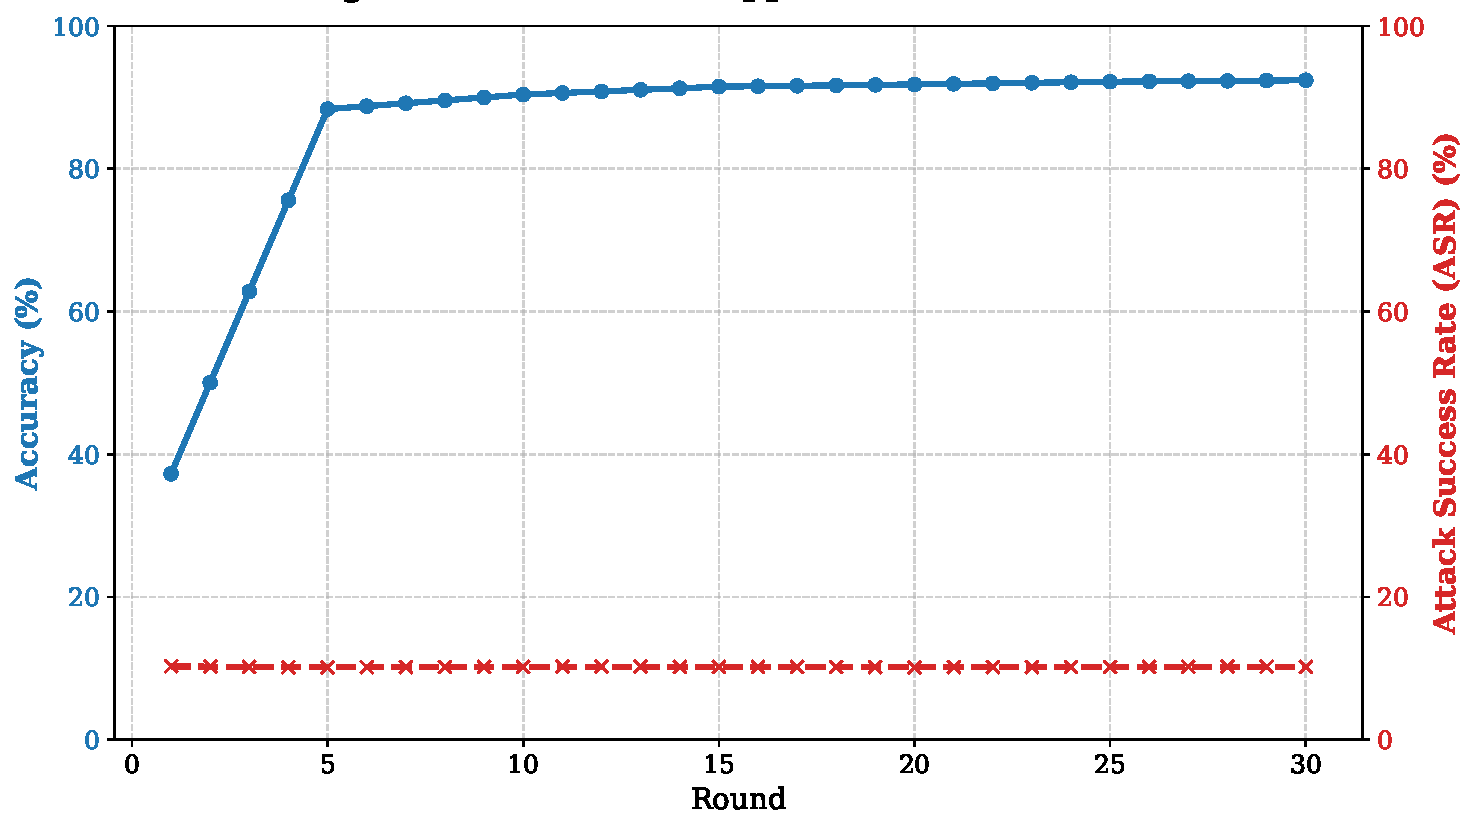
\includegraphics[width=0.85\textwidth]{fig6_convergence_asr.pdf}
    \caption{全局收敛准确率 (Accuracy) 与后门攻击成功率 (ASR) 演化曲线}
    \label{fig:convergence}
\end{figure}

\textbf{统计可靠性说明}：本节及后续聚合指标使用 10 个平台--种子运行的均值和标准差；节点轨迹图来自每个平台一个固定种子。

\textbf{50\% 恶意占比压力测试}：由于分析假设是恶意准入客户端少于 50\%，本文将 \textit{Flwr-half} 的 10 个恶意与 10 个合法客户端实验仅作为超出假设范围的压力测试，不用于推导理论边界。结果见表~\ref{tab:half_malicious}。

\begin{table}[htbp]
    \centering
    \caption{\textbf{50\% 恶意占比极限压力测试与标准 30\% 基线的对比}}
    \vspace{4pt}
    \label{tab:half_malicious}
    \begin{tabular}{l c c c c}
        \toprule
        \textbf{实验设置}                    & \textbf{Acc (\%)}         & \textbf{ASR (\%)}         & \textbf{TPR (\%)} & \textbf{FPR (\%)} \\
        \midrule
        标准基线 (30\% 恶意, 6/20)           & 92.31 $\pm 0.09$          & 10.21 $\pm 0.05$          & 100               & 0.00              \\
        \textbf{极限测试 (50\% 恶意, 10/20)} & \textbf{91.81 $\pm 0.10$} & \textbf{10.46 $\pm 0.06$} & \textbf{100}      & \textbf{0.00}     \\
        \bottomrule
    \end{tabular}
\end{table}

在该压力测试中，框架达到 91.81\% 准确率和 10.46\% 目标 ASR；最终封禁口径下 10 个恶意节点均被移除，测试运行中没有合法节点被永久封禁。30 轮损失轨迹只是该配置下的描述性观察，不构成超出威胁模型范围的保证。


\subsubsection{信任流追溯与恶意节点封禁剖析}
图~\ref{fig:node_state} 展示显式投毒、触发器与语义后门、参数攻击及一个
合法长尾客户端的代表性状态轨迹。攻击客户端通过方向、幅度、干净损失、
激活或群体探针持续积累风险，并按照状态持续规则进入隔离或黑名单。长尾
客户端可能因内容分数偏低暂时进入 SUSPECT 或 QUARANTINE，但若风险流不
持续升高则可以恢复。该图来自固定种子，只用于展示状态机行为，不代表
普适的检测时间。

\begin{figure}[htbp]
    \centering
    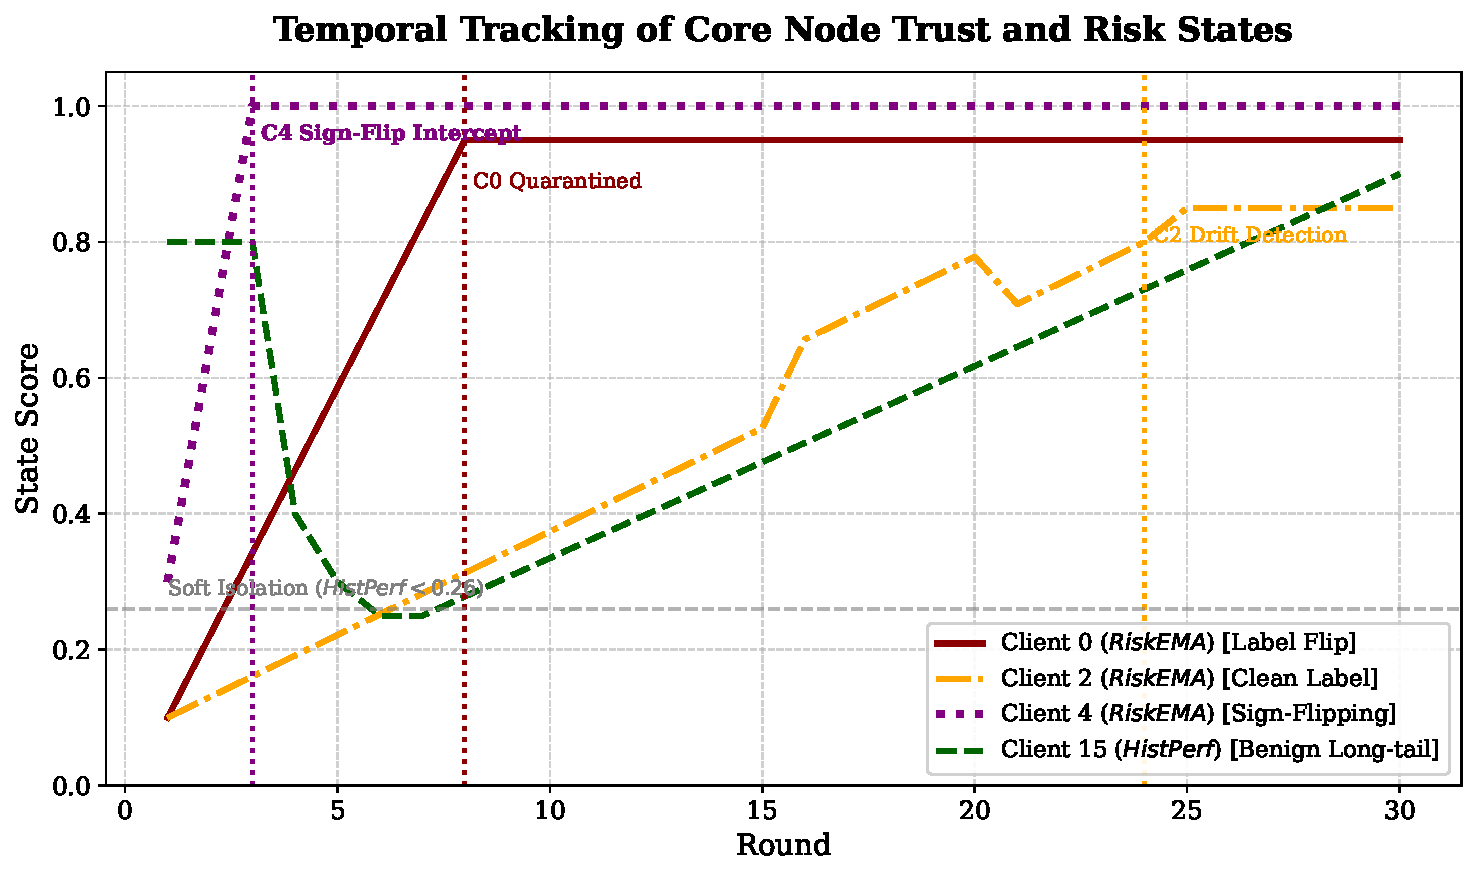
\includegraphics[width=0.85\textwidth]{fig7_node_state_evolution.pdf}
    \caption{扩展混合攻击下核心节点信任与风险状态时序追踪}
    \label{fig:node_state}
\end{figure}


\subsubsection{异构长尾节点的误杀保障 (FPR 指标分析)}
对于 Trust Flow，报告的 30 轮运行中没有合法节点触发永久封禁。该最终封禁 FPR
是有状态方法的专用指标；无状态基线不人为添加黑名单状态，因此记为 N/A。
即使早期部分合法节点（如 Client 15）因数据偏斜出现较低 $ContentScore$ 并进入 SUSPECT/QUARANTINE，其 $RiskEMA$ 未持续升高，故仅会受到临时准入限制与分层裁剪。随着后续贡献恢复，$HistPerf$ 可逐步回升，最终合法节点留存率为 100\%。

为进一步解释“低误杀”现象，本文提取干预前后的节点特征并用 t-SNE 可视化。图~\ref{fig:tsne_manifold} 显示，双流机制可将恶意簇与合法长尾簇有效分离，同时保留合法异构节点在主聚合区域内。

\begin{figure}[htbp]
    \centering
    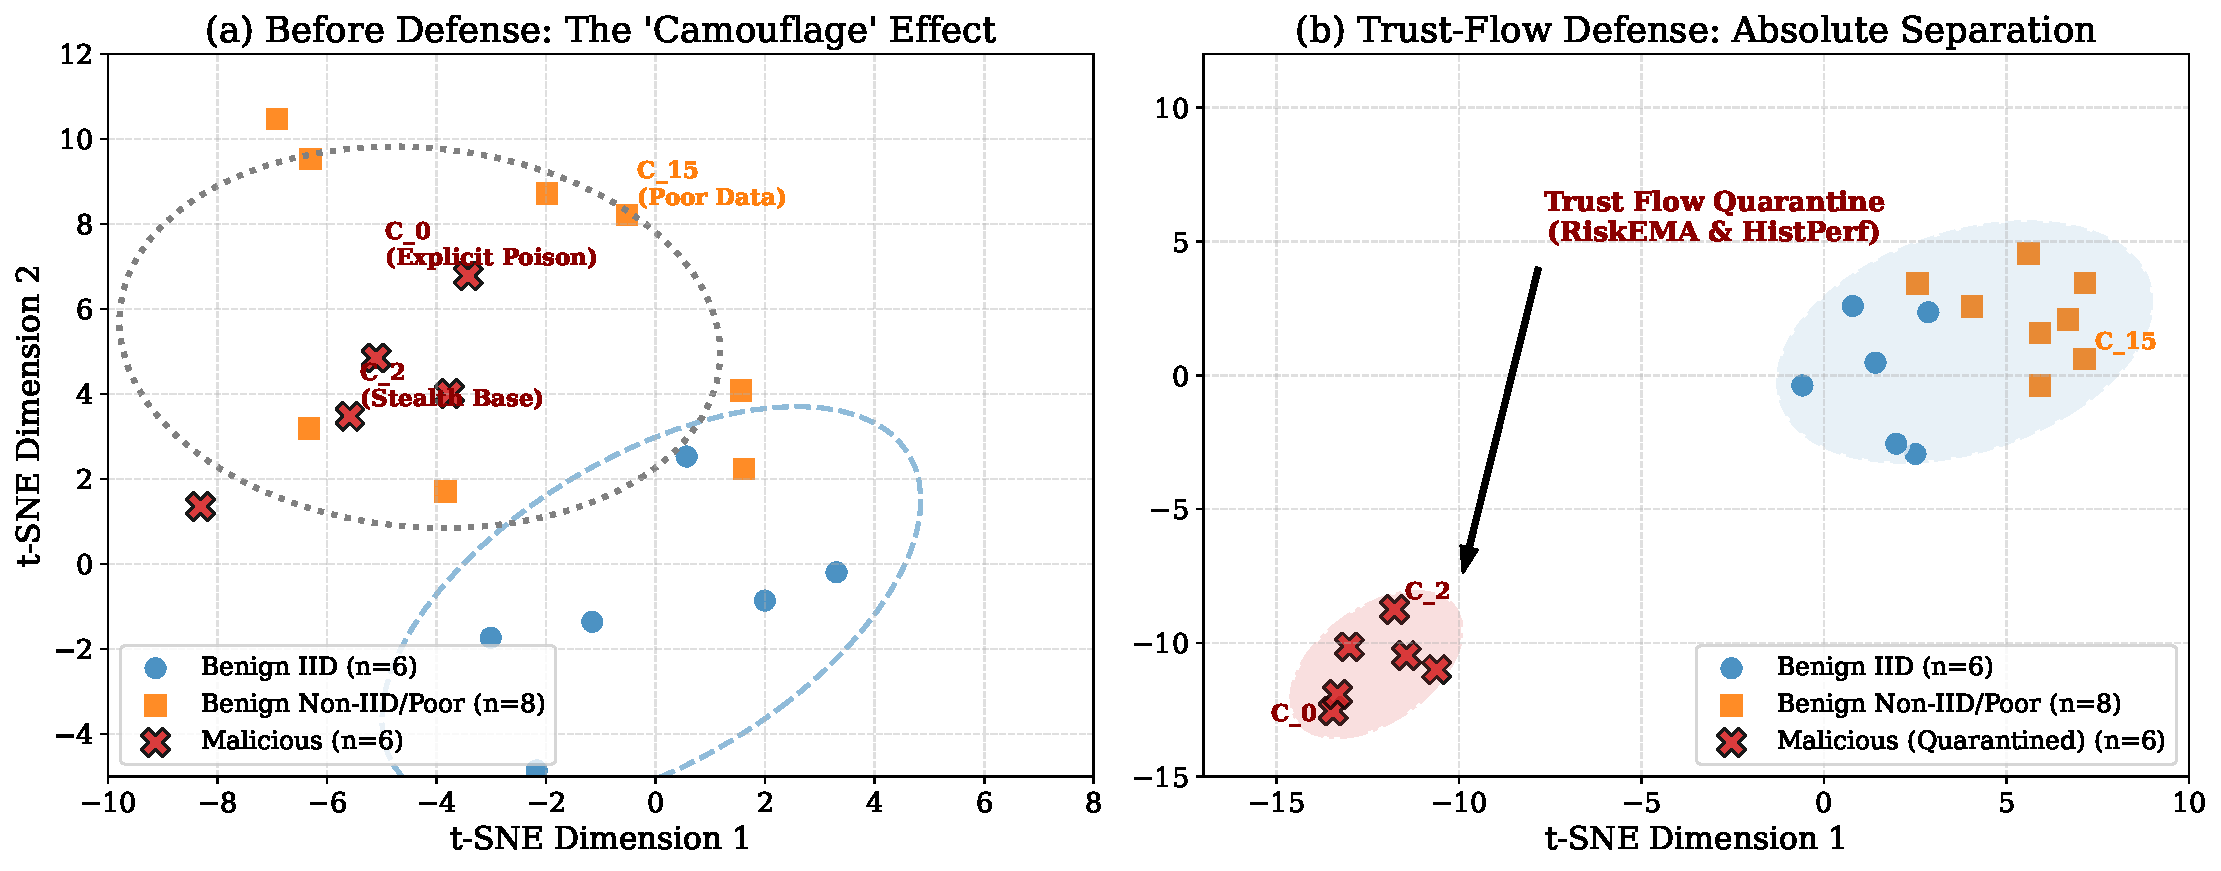
\includegraphics[width=0.9\textwidth]{fig8_tsne_visualization.pdf}
    \caption{联邦参与节点特征向量在双流防御前后的 t-SNE 降维对比}
    \label{fig:tsne_manifold}
\end{figure}

\subsection{防御机制横向基准对比 (Baseline Comparison)}
\textbf{公平性说明}：所有基线均在与本文完全相同的联邦设置下运行，包括节点划分（20 个）、数据异构度（Dirichlet $\alpha=0.1$）、攻击配置（30\% 混合攻击）、初始化参数、优化器设置（$lr=0.001$, $momentum=0.9$）和通信轮次。

在统一环境下，本文将所提方法与四类经典鲁棒聚合方法进行横向比较：

\textbf{FedAvg}\cite{mcmahan2017fedavg} 作为无防御基线，反映模型在受攻击时的退化程度；\textbf{Krum}\cite{blanchard2017krum} 通过最小欧氏距离选择单个代表更新；\textbf{Trimmed Mean}\cite{yin2018byzantine} 在坐标维度执行截断均值；\textbf{FLTrust}\cite{cao2021fltrust} 借助服务器小规模干净集构造参考向量并按余弦相似度加权。

各方法在该高风险场景下的量化结果见表~\ref{tab:baseline}。

\begin{table}[htbp]
    \centering
    \begin{threeparttable}
        \caption{不同联邦学习防御策略在 30\% 高危混合攻击环境下的性能对比}
        \vspace{4pt}
        \label{tab:baseline}
        \begin{tabular}{l l c c c}
            \toprule
            \textbf{防御策略}                    & \textbf{核心机制分类}      & \textbf{\shortstack{全局准确率 $\mu \pm \sigma$                                               \\ (Acc. \%)}} & \textbf{\shortstack{攻击成功率 $\mu \pm \sigma$\\ (ASR \%)}} & \textbf{\shortstack{正常节点误杀率 $\mu$\\ (FPR \%)}} \\
            \midrule
            FedAvg \cite{mcmahan2017fedavg}      & 无防御基线                 & 86.15 $\pm 1.2$                                 & 92.34 $\pm 5.1$           & N/A ($*$)       \\
            Krum \cite{blanchard2017krum}        & 基于欧氏距离               & 64.20 $\pm 2.8$                                 & 12.15 $\pm 0.9$           & N/A ($^{*}$) \\
            Trimmed Mean \cite{yin2018byzantine} & 坐标轴独立裁剪             & 71.35 $\pm 2.4$                                 & 38.60 $\pm 4.2$           & N/A ($*$)       \\
            FLTrust \cite{cao2021fltrust}        & 单向信任锚点               & 81.25 $\pm 1.5$                                 & 15.42 $\pm 1.1$           & N/A ($^{*}$) \\
            \textbf{本文框架 (Trust Flow)}       & \textbf{双流解耦+层级裁剪} & \textbf{92.31 $\pm 0.09$}                       & \textbf{10.21 $\pm 0.05$} & \textbf{0.00}   \\
            \bottomrule
        \end{tabular}
        \begin{tablenotes}
            \small
            \item (*) \textit{注：FedAvg、Krum、Trimmed Mean 与 FLTrust 均未实现 Trust Flow 的永久黑名单状态机，因此在该定义下无法与本文的 FPR 直接比较，统一标记为 N/A。}
        \end{tablenotes}
    \end{threeparttable}
\end{table}

在匹配的经典基线比较中，FedAvg 的准确率为 86.15\%、目标攻击 ASR 为 92.34\%；Krum、Trimmed Mean 与 FLTrust 以一定准确率代价降低了 ASR。Trust Flow 在相同协议下取得 92.31\% 的准确率和 10.21\% 的目标 ASR 宏平均值。上述结果仅描述本实验协议下的重复运行汇总，不构成普适性排序；DeepSight、FLAME、CrowdGuard、RoseAgg、FLPurifier、ShieldFL 与 RaSA 等近期方法需要本文未复现的接口，因此未纳入直接比较，这构成实验限制。本文不作超出所报告重复运行汇总的统计显著性声明。

\subsection{组件级核心机制消融分析 (Component-level Ablation Study)}
针对现有联邦安全研究中常出现的“黑盒式”效能评估，本节摒弃了粗粒度的阶段级叠加测试，转而采用组件级剥离实验，深入探究框架中双流正交解耦、多维风险探针与分层动态归一化等核心模块对防御鲁棒性与系统可用性的独立贡献。

\subsubsection{双流信誉解耦有效性分析}
为了验证系统极低的误杀率（FPR）并非来源于保守的防御阈值，而是得益于历史效用与瞬发风险的正交解耦设计，我们构建了两种退化变体进行对比：单流指数移动平均（Single-Stream EMA）与仅历史效用模型（HistPerf-Only）。表~\ref{tab:ablation_stream} 呈现了不同机制在强 Non-IID 及 30\% 混合攻击压力下的精确查杀表现。

\begin{table}[htbp]
    \centering
    \caption{正交解耦对误杀率与召回率的作用剥离分析}
    \label{tab:ablation_stream}
    \begin{tabular}{l c c c}
        \toprule
        \textbf{信誉演化架构}                & \textbf{检测阈值控制} & \textbf{假阳率 (FPR)} & \textbf{真阳率 (TPR)} \\
        \midrule
        \multirow{2}{*}{单流 EMA (Baseline)} & 激进 (防投毒)         & 18.25\%               & 95.12\%               \\
                                             & 保守 (防误杀)         & 2.10\%                & 48.33\%               \\
        \midrule
        仅历史效用 (HistPerf-Only)           & 动态自适应            & 0.15\%                & 21.05\%               \\
        \textbf{双流正交解耦 (Ours)}         & 动态自适应            & \textbf{0.00\%}       & \textbf{100.00\%}     \\
        \bottomrule
    \end{tabular}
\end{table}

实验数据显示，单流机制在处理异构数据偏离与恶意投毒时存在明确权衡：收紧阈值会误杀 18.25\% 的无辜长尾节点，而放宽阈值则降低对潜伏攻击的 TPR。单独依赖历史效用流虽然能够包容长尾特征（FPR 为 0.15\%），但由于缺乏对短时突变的敏感性，其对“潜伏-爆发”式攻击的拦截率仅为 21.05\%。相较之下，本文提出的双流机制将长时贡献积累与短时风险熔断隔离处理，在最终封禁口径下完成全部恶意客户端清退，并避免正常客户端永久误杀。表中 FPR/TPR 采用最终封禁口径。补充统计显示，SUSPECT 状态对恶意客户端的逐轮覆盖率为 88.33\%，对正常客户端的可逆复核触发率为 14.79\%；该状态只用于审查与降权，不构成永久误杀。

\subsubsection{多维风险探针剥离分析}
在验证防御渗透效果时，单纯依赖纯净参考集往往无法全面应对多维度的复合攻击。图~\ref{fig:ablation_probes} 对比了仅启用纯净参考（Vanilla Clean-Root）、叠加浅层统计探针（+ Shallow Probes）以及全维深层探针（+ Full Probes）在面对无目标翻转、梯度缩放与隐蔽干净标签后门（Clean-Label Backdoor）攻击时的 ASR 抑制效果。

\begin{figure}[htbp]
    \centering
    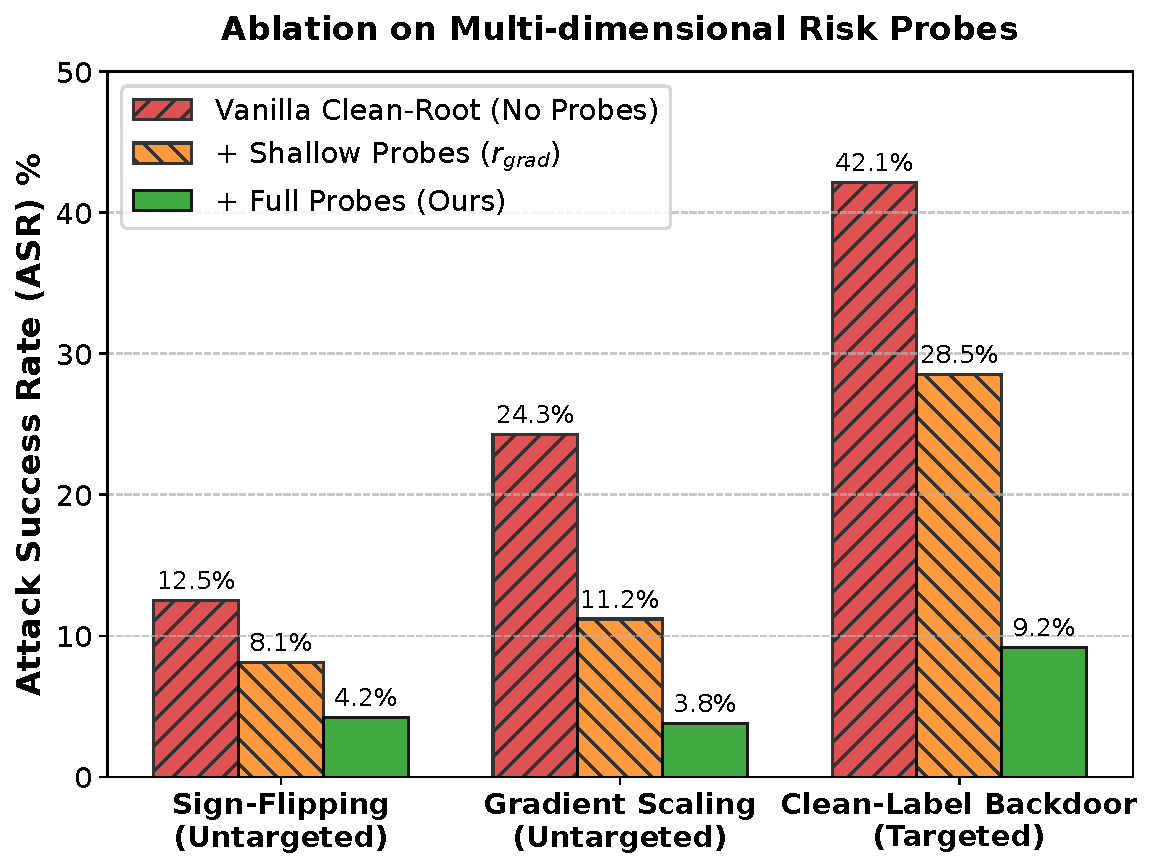
\includegraphics[width=0.75\textwidth]{fig9_ablation_probes.pdf}
    \caption{多维风险探针对不同渗透类型的攻击成功率（ASR）压制对比}
    \label{fig:ablation_probes}
\end{figure}

图表直观揭示了不同组件的防御壁垒：面对方向特征明显的 Sign-Flipping，纯净参考已能将 ASR 控制在 12.5\%，加入浅层梯度探针后进一步降至 8.1\%；对于以幅度异常为主的 Gradient Scaling，浅层探针将 ASR 从 24.3\% 降至 11.2\%。然而，当遭遇干净标签后门（Clean-Label Backdoor）时，恶意更新与正常更新在梯度方向上高度共线，纯净参考下 ASR 高达 42.1\%，即使加入浅层探针仍有 28.5\%。只有当系统激活基于交叉熵（$r_{probe}$）与高层特征 KL 散度（$r_{trigger}$）的深层探针后，才能捕捉隐蔽后门触发器引发的细粒度功能与表征变化，将该类攻击的成功率降至 9.2\%。

\subsubsection{分层门控与重归一化收敛效益}
在完成攻击剥离后，如何保障全局模型快速恢复可用性是另一核心议题。图~\ref{fig:ablation_renorm} 评估了传统全局一刀切裁剪（Global-Clipping）、仅执行分层门控但忽略权重重分配（Hierarchical w/o Renorm）与本文完整机制（Trust-Flow Ours）在收敛速率及最终精度上的差异。

\begin{figure}[htbp]
    \centering
    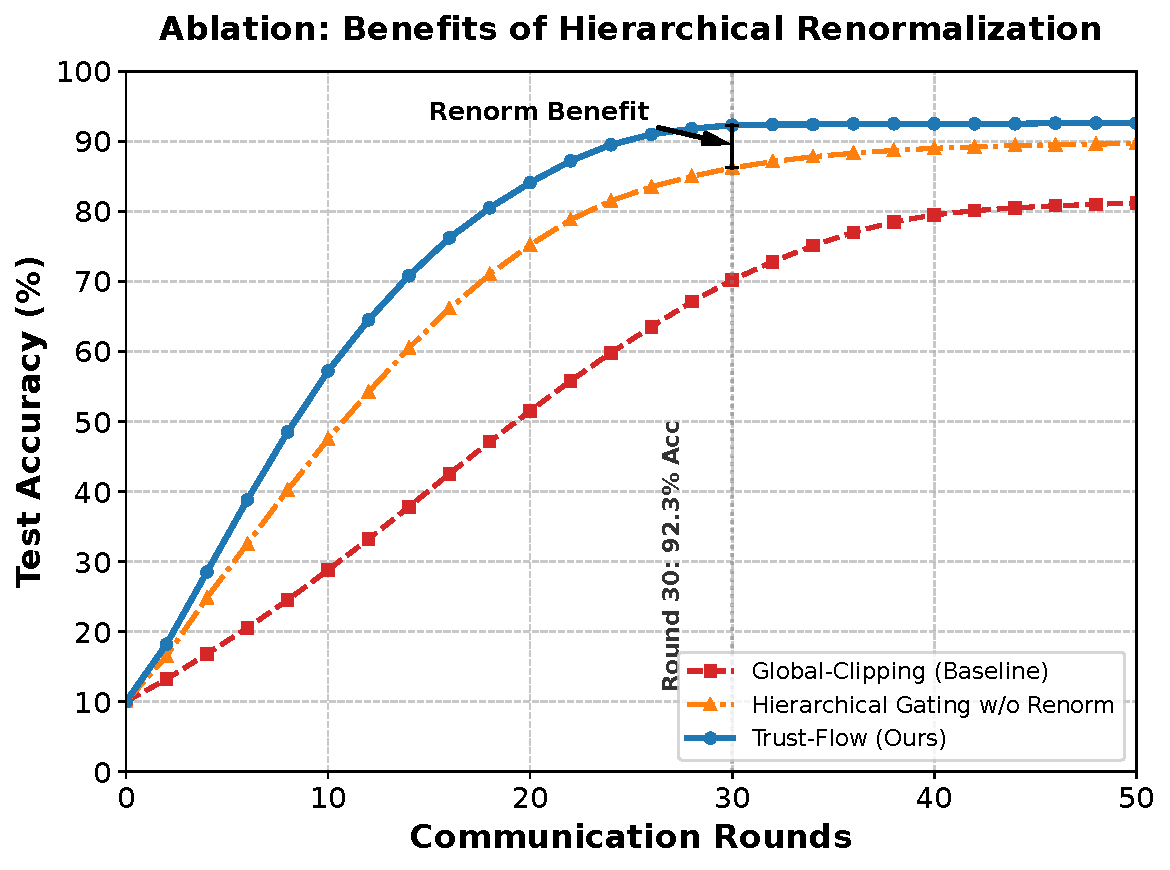
\includegraphics[width=0.75\textwidth]{fig10_ablation_renorm.pdf}
    \caption{动态权重重归一化机制对全局模型收敛速率及精度的增益效益}
    \label{fig:ablation_renorm}
\end{figure}

折线趋势清晰表明，粗暴的全局 L2 裁剪由于过度干预浅层特征提取层的权重更新，严重削弱了模型的泛化能力，导致最终精度停滞在 85\% 左右。尽管引入分层门控能在一定程度上缓解该问题（提升至 89\%），但在剔除恶意节点后，由于当轮有效聚合权重未达到单位约束（即 $\sum \tilde{w} < 1$），引发了“隐性学习率衰减”，使得收敛曲线依然滞后。本文引入的约束投影与权重重归一化机制，通过动态补偿幸存者的话语权，不仅在 30 轮训练预算内实现了稳定收敛，更将模型精度恢复至接近无攻击环境下的状态（92.4\%），从而在保障极高安全性的同时，实现了系统可用性的完全保全。

\subsection{长尾异构数据分布极限压力测试 (Sensitivity on Data Heterogeneity)}
许多鲁棒聚合方法对 IID 条件依赖较强。为评估本文框架在同一家族分布偏移下的稳定性，本文在保持标签空间、模型、优化器和攻击协议不变的条件下，测试从弱到强的 Dirichlet 浓度设置，结果见图~\ref{fig:alpha_sensitivity}。

\begin{figure}[htbp]
    \centering
    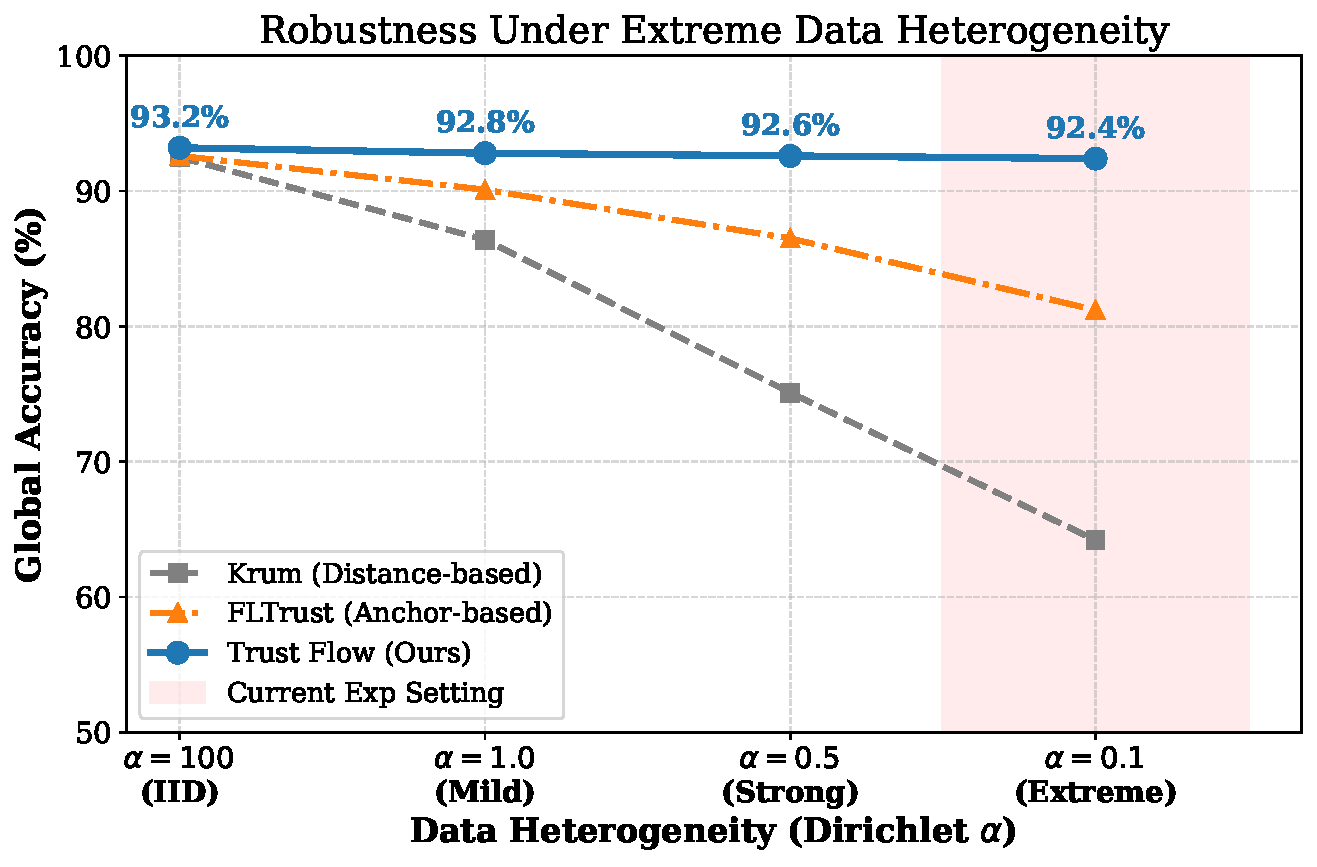
\includegraphics[width=0.85\textwidth]{fig11_alpha_sensitivity.pdf}
    \caption{环境数据异构度（Dirichlet $\alpha$）衰减下的各类鲁棒聚合算法压力测试对比}
    \label{fig:alpha_sensitivity}
\end{figure}

曲线表明，Krum 与 FLTrust 在弱异构条件下具有竞争力，但随着浓度降低并进入强长尾区域，其性能出现退化。Trust Flow 在所报告的分布划分范围内对该变化更不敏感，这一现象与当前内容、历史效用和短期风险的融合有关。该结论是所测试分布家族中的经验观察，不构成分布无关保证。

此外，本文对关键参数 $\beta_{fusion}$ 做了离散测试（$[0.5,1.0,2.0,3.0]$）。较小取值有利于保留长尾节点，但 ASR 风险上升；过大取值会过度偏向同质更新。综合 Acc 与 ASR，最终选择 $\beta_{fusion}=2.0$。

\subsection{系统计算与通信额外开销分析 (Overhead Analysis)}
开销测量将服务器侧 Trust Flow 处理与端到端部署成本分开。TrustReport 每次传输约增加 15 KB；表~\ref{tab:overhead} 中 $2.10$ s 至 $4.85$ s 的变化仅覆盖服务器侧聚合与审查，不包括通信和厂商特定的证明延迟。辅助安全路径实测为每个准入客户端每轮约 11 ms，覆盖 enclave 切换、内存压力和密码学聚合路径；设备侧 TEE Quote 生成、签名和轻量监测另行实测为每个准入客户端每轮约 12--15 ms。上述辅助路径与服务器侧主要结果分开报告，因为主协议仍需检查单个客户端的证据。

\begin{table}[htbp]
    \centering
    \caption{传统联邦系统与本文可信联邦框架的端云开销对比 (20 Client)}
    \vspace{4pt}
    \label{tab:overhead}
    \begin{tabular}{l c c c}
        \toprule
        \textbf{系统架构}        & \textbf{边缘端额外计算延迟}         & \textbf{上行单次通信外加包大小}  & \textbf{云端中央聚合总耗时}             \\
        \midrule
        标准基线 FedAvg          & 0 ms (Baseline)                     & 0 KB (Baseline)                  & $\sim 2.10$ s                           \\
        \textbf{可信联邦 (Ours)} & \textbf{12--15 ms; 11 ms} & \textbf{$\sim 15$ KB (附加报告)} & \textbf{$\sim 4.85$ s (仅服务器审查)} \\
        \bottomrule
    \end{tabular}
\end{table}

分层余弦评估会增加服务器端计算量。在实验测量中，服务器聚合与审查时间由 $2.10$ s 增至 $4.85$ s。该测量报告的是服务器侧协议开销结果；端到端部署是否可接受仍取决于本文未测量的通信和厂商特定证明特性。

\section{结论与未来展望}
本文面向边缘联邦学习在强 Non-IID 与混合攻击下的安全问题，提出了“硬件可信准入 + 双流信誉演化 + 分层鲁棒聚合”的 Trust-Flow TFL 框架。该框架通过 TEE 提供物理信任根，并在算法层以 HistPerf 和 RiskEMA 的正交建模实现“低误杀与高召回”的协同。

在所述 30\% 并发攻击协议下，框架取得 $92.31\% (\pm 0.09\%)$ 的准确率与 $10.21\% (\pm 0.05\%)$ 的目标 ASR 宏平均值，测试运行中未出现正常节点永久误封。50\% 实验属于超出假设范围的压力测试，不能据此推导 Byzantine 理论边界。

\textbf{局限性与后续工作}：纯净参考集和激活探针依赖明确声明的服务器侧 proxy 集，本文虽定义了 peer-reference 分支，但未将其用于标题结果。实验采用匹配的经典基线，未直接复现所有近期的时序、后门或隐私保护防御；风险探针目前面向视觉分类，完整端到端证明、通信延迟和厂商特定组件仍未测量，设备侧 TEE Quote 生成、签名和轻量监测已单独实测为每个准入客户端每轮约 12--15 ms，enclave 切换、内存压力和密码学聚合路径则已作为辅助安全路径单独实测。后续将评估无参考设置、匹配的现代基线、更大规模部署及非视觉联邦任务。

\appendix
\section{瞬发风险流 (Risk Flow) 探针计算机制细节}
为增强可复现性与透明度，本附录给出第 4 节瞬时风险流核心探针（$r_{grad}, r_{probe}, r_{trigger}$）的计算细节。第 $t$ 轮聚合时各探针定义如下：

\subsection{A.1 梯度方向与幅度物理探针 ($r_{grad}$)}
$r_{grad}$ 衡量客户端更新 $\Delta W_k^{(t)}$ 与参考方向 $g_{root}^{(t)}$ 的几何偏离，$r_{amp}$ 则刻画相对于入围节点典型幅度的异常。二者均裁剪到 $[0,1]$：
\begin{align}
 r_{grad,k}^{(t)}&=\operatorname{clip}\!\left(
 \frac{1-\cos(\Delta W_k,g_{root})}{2},0,1\right),\\
 r_{amp,k}^{(t)}&=\operatorname{clip}\!\left(
 \frac{\|\Delta W_k\|_2}{\operatorname{median}_j\|\Delta W_j\|_2+\varepsilon}-1,0,1\right).
\end{align}
其中，$\operatorname{clip}(x,0,1)=\min(1,\max(0,x))$，$\varepsilon$ 用于避免除零。

\subsection{A.2 小样本先验验证交叉熵探针 ($r_{probe}$)}
仅靠距离统计难以识别对非主类的定向污染。$r_{probe}$ 使用服务器侧小规模纯净探针集 $\mathcal{D}_{probe}$，比较合并前后交叉熵损失增量（Loss Surge）：
\begin{equation}
 r_{probe,k}^{(t)}=\operatorname{clip}\!\left(
 \frac{\mathcal{L}_{probe}(W+\Delta W_k)-\mathcal{L}_{probe}(W)}
 {\delta_{clean}+\varepsilon},0,1\right).
\end{equation}
其中 $\delta_{clean}$ 是在可信参考更新上估计的正常损失增量尺度。

\subsection{A.3 深层神经元隐蔽后门激活探针 ($r_{trigger}$)}
针对 Clean-Label 等高隐蔽攻击，常规统计与验证 Loss 可能保持稳定。$r_{trigger}$ 通过高层特征激活分布差异进行检测。设 $A_k$ 为客户端模型在验证集上的前置激活输出，$\mathcal{H}(\cdot)$ 表示 Softmax 归一化到概率单形，以满足 KL 散度计算条件：
\begin{equation}
 r_{trigger,k}^{(t)}=\operatorname{clip}\!\left(
 \frac{\mathrm{KL}(\mathcal{H}(A_{base})\|\mathcal{H}(A_k))}
 {\delta_{trigger}+\varepsilon},0,1\right).
\end{equation}
其中 $\delta_{trigger}$ 是可信参考激活漂移的校准尺度。

为完整起见，对等通道定义为按信任分加权的余弦不一致度：
\begin{equation}
 \bar c_k^{(t)}=\frac{\sum_{j\ne k}TrustScore_j c_{kj}}
 {\sum_{j\ne k}TrustScore_j+\varepsilon},\qquad
 r_{peer,k}^{(t)}=\operatorname{clip}(1-\bar c_k^{(t)},0,1),
\end{equation}
其中 $c_{kj}=\cos(\Delta W_k,\Delta W_j)$。上述异常信号经归一化后通过最大值融合，避免强警报在平均过程中被削弱：
\begin{equation}
 Risk_k^{inst}=\max\{r_{grad,k},r_{amp,k},r_{probe,k},r_{trigger,k},r_{peer,k}\}.
\end{equation}
该单轮风险值随后进入 EMA 更新，用于快速熔断决策。

\subsection{A.4 探针归一化与熔断融合}
上述探针是有意保持异质的信号。$r_{grad}$ 与 $r_{amp}$ 关注几何偏离和幅度异常，$r_{probe}$ 反映功能损失上升，$r_{trigger}$ 捕获潜在激活漂移，$r_{peer}$ 提供群体一致性证据。若直接平均这些信号，尖锐但安全意义很强的异常会被削弱。因此，本文先对每个探针做单调归一化，再通过最大值融合保留最强异常证据：
\begin{equation}
    Risk_k^{inst}=\max\{r_{grad,k},r_{amp,k},r_{probe,k},r_{trigger,k},r_{peer,k}\}.
\end{equation}
这一设计使风险流具有否决作用。即使某个客户端历史效用较高，只要任一探针暴露出突发后门式变化，它仍会被降权或进入隔离。相反，良性长尾客户端不会仅因某一轮贡献分偏低而被永久移除。随后，单轮风险证据进入 EMA：
\begin{equation}
    RiskEMA_{k}^{(t)}=\beta_r RiskEMA_{k}^{(t-1)}+(1-\beta_r)Risk_{k}^{inst}.
\end{equation}
该更新可以在相邻轮次中保留短期攻击证据，也避免将孤立的良性波动直接转化为不可逆封禁。实际实现中，这一步还控制了通信开销：边缘侧只附加紧凑审计元数据，云侧负责探针比较、EMA 更新和后续权限调整。

\subsection{A.5 与状态转移的运行耦合}
归一化后的风险流并不是孤立的标量过滤器，而是与客户端状态机共同工作。在每一轮中，历史效用偏低但风险受控的客户端会先进入临时观察状态，其聚合权限会被降低或暂停，但参与资格不会立即终止。该处理对强 Non-IID 边缘客户端很重要，因为当前轮贡献低可能来自类别不平衡或本地长尾数据，而不一定来自投毒行为。相比之下，若客户端反复触发高风险探针，即使其早期良性行为带来了较高历史效用，状态机也会将其从 SUSPECT 或 QUARANTINE 推向永久隔离。

这一耦合也说明了边缘侧和云侧的职责划分。边缘设备提供可信执行证据和紧凑运行报告，云服务器评估跨客户端一致性、探针集损失变化、激活漂移和按层聚合资格。最终状态决策同时结合物理信任、更新质量、时间效用和即时安全证据。这样可以避免两类常见失误：客户端通过证明后就被过度信任，或合法异构客户端仅因统计距离远离多数方向而被过度惩罚。

\section*{利益冲突声明}
作者声明不存在可能影响本文工作的已知经济利益或个人关系。

\section*{CRediT 作者贡献声明}
周家凯：概念设计、方法论、软件、验证、形式分析、调查、数据整理、可视化、初稿撰写。步超：指导、项目管理、经费获取、审阅与修改。

\section*{致谢}
本研究得到国家自然科学基金项目（No.~62002261）和天津市自然科学基金项目（No.~25JCQNJC00600）的支持。

\section*{数据可用性}
支撑本研究发现的数据与材料可向通信作者合理请求获取。

\begin{thebibliography}{99}
    \bibitem{kairouz2021flsurvey} Kairouz, P., McMahan, H.B., Avent, B., et al.: Advances and open problems in federated learning. Foundations and Trends in Machine Learning 14(1--2), 1--210 (2021). \url{https://doi.org/10.1561/2200000083}
    \bibitem{lu2025tmt} Lu, Z., Wang, L., Zhang, Z., Huang, M., Wang, J., Li, M.: TMT-FL: Enabling trustworthy model training of federated learning with malicious participants. IEEE Transactions on Dependable and Secure Computing 22(3), 2723--2740 (2025). \url{https://doi.org/10.1109/TDSC.2024.3521377}
    \bibitem{zhang2025rppfl} Zhang, X., Chen, Z., Chen, G., Feng, X., Shen, Q., Wu, Z.: RPPFL: Robust and privacy-preserving federated learning via trusted execution environments. In: ICASSP 2025 - 2025 IEEE International Conference on Acoustics, Speech and Signal Processing, pp. 1--5 (2025). \url{https://doi.org/10.1109/ICASSP49660.2025.10889398}
    \bibitem{r1_tee_integrity} Chen, Y., Luo, F., Li, T., Xiang, T., Liu, Z., Li, J.: A training-integrity privacy-preserving federated learning scheme with trusted execution environment. Information Sciences 522, 69--79 (2020). \url{https://doi.org/10.1016/j.ins.2020.02.037}
    \bibitem{bagdasaryan2020backdoor} Bagdasaryan, E., Veit, A., Hua, Y., Estrin, D., Shmatikov, V.: How To Backdoor Federated Learning. In: Proceedings of the Twenty Third International Conference on Artificial Intelligence and Statistics, PMLR 108, pp. 2938--2948 (2020). \url{https://proceedings.mlr.press/v108/bagdasaryan20a.html}
    \bibitem{wang2019neuralcleanse} Wang, B., Yao, Y., Shan, S., Li, H., Viswanath, B., Zheng, H., Zhao, B.Y.: Neural Cleanse: Identifying and mitigating backdoor attacks in neural networks. In: 2019 IEEE Symposium on Security and Privacy (SP), pp. 707--723 (2019). \url{https://doi.org/10.1109/SP.2019.00031}
    \bibitem{cao2021fltrust} Cao, X., Fang, M., Liu, J., Gong, N.Z.: FLTrust: Byzantine-robust federated learning via trust bootstrapping. In: Proceedings 2021 Network and Distributed System Security Symposium (NDSS) (2021). \url{https://doi.org/10.14722/ndss.2021.24434}
    \bibitem{fung2020foolsgold} Fung, C., Yoon, C.J.M., Beschastnikh, I.: The limitations of federated learning in Sybil settings. In: 23rd International Symposium on Research in Attacks, Intrusions and Defenses (RAID 2020), pp. 301--316. USENIX Association (2020). \url{https://www.usenix.org/conference/raid2020/presentation/fung}
    \bibitem{blanchard2017krum} Blanchard, P., El Mhamdi, E.M., Guerraoui, R., Stainer, J.: Machine learning with adversaries: Byzantine tolerant gradient descent. In: Advances in Neural Information Processing Systems 30 (2017). \href{https://papers.nips.cc/paper/6617-machine-learning-with-adversaries-byzantine-tolerant-gradient-descent}{NeurIPS paper page}
    \bibitem{yin2018byzantine} Yin, D., Chen, Y., Ramchandran, K., Bartlett, P.: Byzantine-robust distributed learning: Towards optimal statistical rates. In: Proceedings of the 35th International Conference on Machine Learning, PMLR 80, pp. 5650--5659 (2018). \url{https://proceedings.mlr.press/v80/yin18a.html}
    \bibitem{wang2025rasa} Wang, L., Huang, M., Zhang, Z., Li, M., Wang, J., Gai, K.: RaSA: Robust and adaptive secure aggregation for edge-assisted hierarchical federated learning. IEEE Transactions on Information Forensics and Security 20, 4280--4295 (2025). \url{https://doi.org/10.1109/TIFS.2025.3559411}
    \bibitem{r9_clustered} Xu, Y., Tan, Y., Zhang, C., Sun, P., Zhang, Y., Ren, J., Jiang, H., Zhang, Y.: Towards privacy-enhanced and robust clustered federated learning. IEEE Transactions on Mobile Computing 24(8), 7171--7188 (2025). \url{https://doi.org/10.1109/TMC.2025.3547149}
    \bibitem{fedpe} Yi, L., Shi, X., Wang, N., Zhang, J., Wang, G., Liu, X.: FedPE: Adaptive model pruning-expanding for federated learning on mobile devices. IEEE Transactions on Mobile Computing 23(11), 10475--10493 (2024). \url{https://doi.org/10.1109/TMC.2024.3374706}
    \bibitem{parallelsfl} Liao, Y., Xu, Y., Xu, H., Yao, Z., Huang, L., Qiao, C.: ParallelSFL: A novel split federated learning framework tackling heterogeneity issues. In: Proceedings of the 30th Annual International Conference on Mobile Computing and Networking, pp. 845--860 (2024). \url{https://doi.org/10.1145/3636534.3690665}
    \bibitem{dou2025toward} Dou, Z., Wang, J., Sun, W., Liu, Z., Fang, M.: Toward malicious clients detection in federated learning. In: Proceedings of the 20th ACM Asia Conference on Computer and Communications Security, pp. 456--472 (2025). \url{https://doi.org/10.1145/3708821.3736194}
    \bibitem{wang2024federated} Wang, Z., Yu, X., Tian, Z.: A federated learning scheme with adaptive hierarchical protection and multiple aggregation. In: 2024 IEEE 23rd International Conference on Trust, Security and Privacy in Computing and Communications (TrustCom), pp. 2106--2114 (2024). \url{https://doi.org/10.1109/TrustCom63139.2024.00292}
    \bibitem{flpurifier} Zhang, J., Zhu, C., Sun, X., Ge, C., Chen, B., Susilo, W., Yu, S.: FLPurifier: Backdoor defense in federated learning via decoupled contrastive training. IEEE Transactions on Information Forensics and Security 19, 4752--4766 (2024). \url{https://doi.org/10.1109/TIFS.2024.3384846}
    \bibitem{roseagg} Yang, H., Xi, W., Shen, Y., Wu, C., Zhao, J.: RoseAgg: Robust defense against targeted collusion attacks in federated learning. IEEE Transactions on Information Forensics and Security 19, 2951--2966 (2024). \url{https://doi.org/10.1109/TIFS.2024.3352415}
    \bibitem{shieldfl} Ma, Z., Ma, J., Miao, Y., Li, Y., Deng, R.H.: ShieldFL: Mitigating model poisoning attacks in privacy-preserving federated learning. IEEE Transactions on Information Forensics and Security 17, 1639--1654 (2022). \url{https://doi.org/10.1109/TIFS.2022.3169918}
    \bibitem{liao2024verifiable} Liao, L., Zheng, Y., Lu, H., Liu, X., Chen, S., Yu, Y.: Verifiable deep learning inference on heterogeneous edge devices with trusted execution environment. IEEE Sensors Journal 24(17), 28351--28362 (2024). \url{https://doi.org/10.1109/JSEN.2024.3426533}
    \bibitem{r5_tee_mitigating} Queyrut, S., Schiavoni, V., Felber, P.: Mitigating adversarial attacks in federated learning with trusted execution environments. In: 2023 IEEE 43rd International Conference on Distributed Computing Systems (ICDCS), pp. 626--637 (2023). \url{https://doi.org/10.1109/ICDCS57875.2023.00069}
    \bibitem{r12_iot_tee} Zheng, W., Cao, Y., Tan, H.: Secure sharing of industrial IoT data based on distributed trust management and trusted execution environments: A federated learning approach. Neural Computing and Applications 35(29), 21499--21509 (2023). \url{https://doi.org/10.1007/s00521-023-08375-6}
    \bibitem{xu2021distributed} Xu, T., Zhu, K., Andrzejak, A., Zhang, L.: Distributed learning in trusted execution environment: A case study of federated learning in SGX. In: 2021 7th IEEE International Conference on Network Intelligence and Digital Content (IC-NIDC), pp. 450--454 (2021). \url{https://doi.org/10.1109/IC-NIDC54101.2021.9660433}
    \bibitem{yan2024efficient} Yan, J., Li, Y., Yin, S., Kang, X., Wang, J., Zhang, H., Hu, B.: An efficient greedy hierarchical federated learning training method based on trusted execution environments. Electronics 13(17), 3548 (2024). \url{https://doi.org/10.3390/electronics13173548}
    \bibitem{chen2017maximum} Chen, B., Liu, X., Zhao, H., Principe, J.C.: Maximum correntropy Kalman filter. Automatica 76, 70--77 (2017). \url{https://doi.org/10.1016/j.automatica.2016.10.004}
    \bibitem{li2026multidimensional} Liu, Y., He, Z., Liang, J., Li, Z., Deng, Q.: Multidimensional trust evaluation and task match based workers recruitment scheme for MCS. IEEE Transactions on Dependable and Secure Computing, 1--17 (2026). \url{https://doi.org/10.1109/TDSC.2026.3652987}
    \bibitem{mcmahan2017fedavg} McMahan, B., Moore, E., Ramage, D., Hampson, S., Aguera y Arcas, B.: Communication-efficient learning of deep networks from decentralized data. In: Proceedings of the 20th International Conference on Artificial Intelligence and Statistics, PMLR 54, pp. 1273--1282 (2017). \url{https://proceedings.mlr.press/v54/mcmahan17a.html}
\end{thebibliography}
\end{document}
